\chapter{SYSTEM DESIGN}



\section{System architecture}

\section{UI/UX design}

In this section, we delve into the UI/UX design for our pet adoption website. Each page has been crafted to enhance user engagement and streamline the adoption process. Begins on the homepage, where users are welcomed with an intuitive interface that serves as the gateway to the platform. The login and register pages provide a seamless onboarding experience, ensuring a secure and personalized environment. The pet search page facilitates effortless exploration, allowing users to discover potential companions with ease. Detailed pet profiles showcase comprehensive information, fostering informed decision-making. The user profile page ensures a tailored experience, while the blog homepage and pages provide valuable insights and updates. To navigate this cohesive ecosystem, a diagram illustrates the interconnectedness of each page, illuminating the user's journey from entry to adoption. To enhance clarity, we've included a comprehensive diagram illustrating the intricate connections between these pages
\subsection{Front office}

\begin{figure}[H]
    \centering
    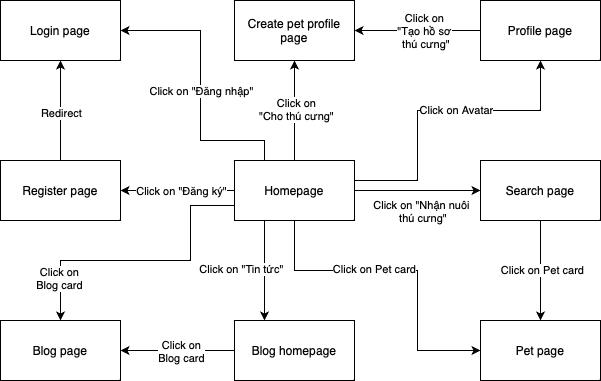
\includegraphics[width=0.8\textwidth]{Figures/wireframe_fo.png}
    \caption{Wireframe for Front office}
\end{figure}

\subsubsection{Homepage}

The homepage serves as the focal point of our pet adoption website, designed with a user-centric approach to ensure an intuitive and engaging experience. The navigation bar stands as a gateway to key functionalities, allowing users to seamlessly register, log in, explore pet profiles, create their pet profiles, access insightful blog content, and manage their user profile. The strategic placement of these navigation options facilitates effortless interaction. The hero section captures attention with visually appealing imagery and succinct messaging, encapsulating the essence of our mission. The "About Us" section provides a deeper understanding of our organization, building trust and connection with our audience. Additionally, the organization section offers insights into our partners and collaborators, fostering a sense of community.

\begin {figure}[H]
\centering
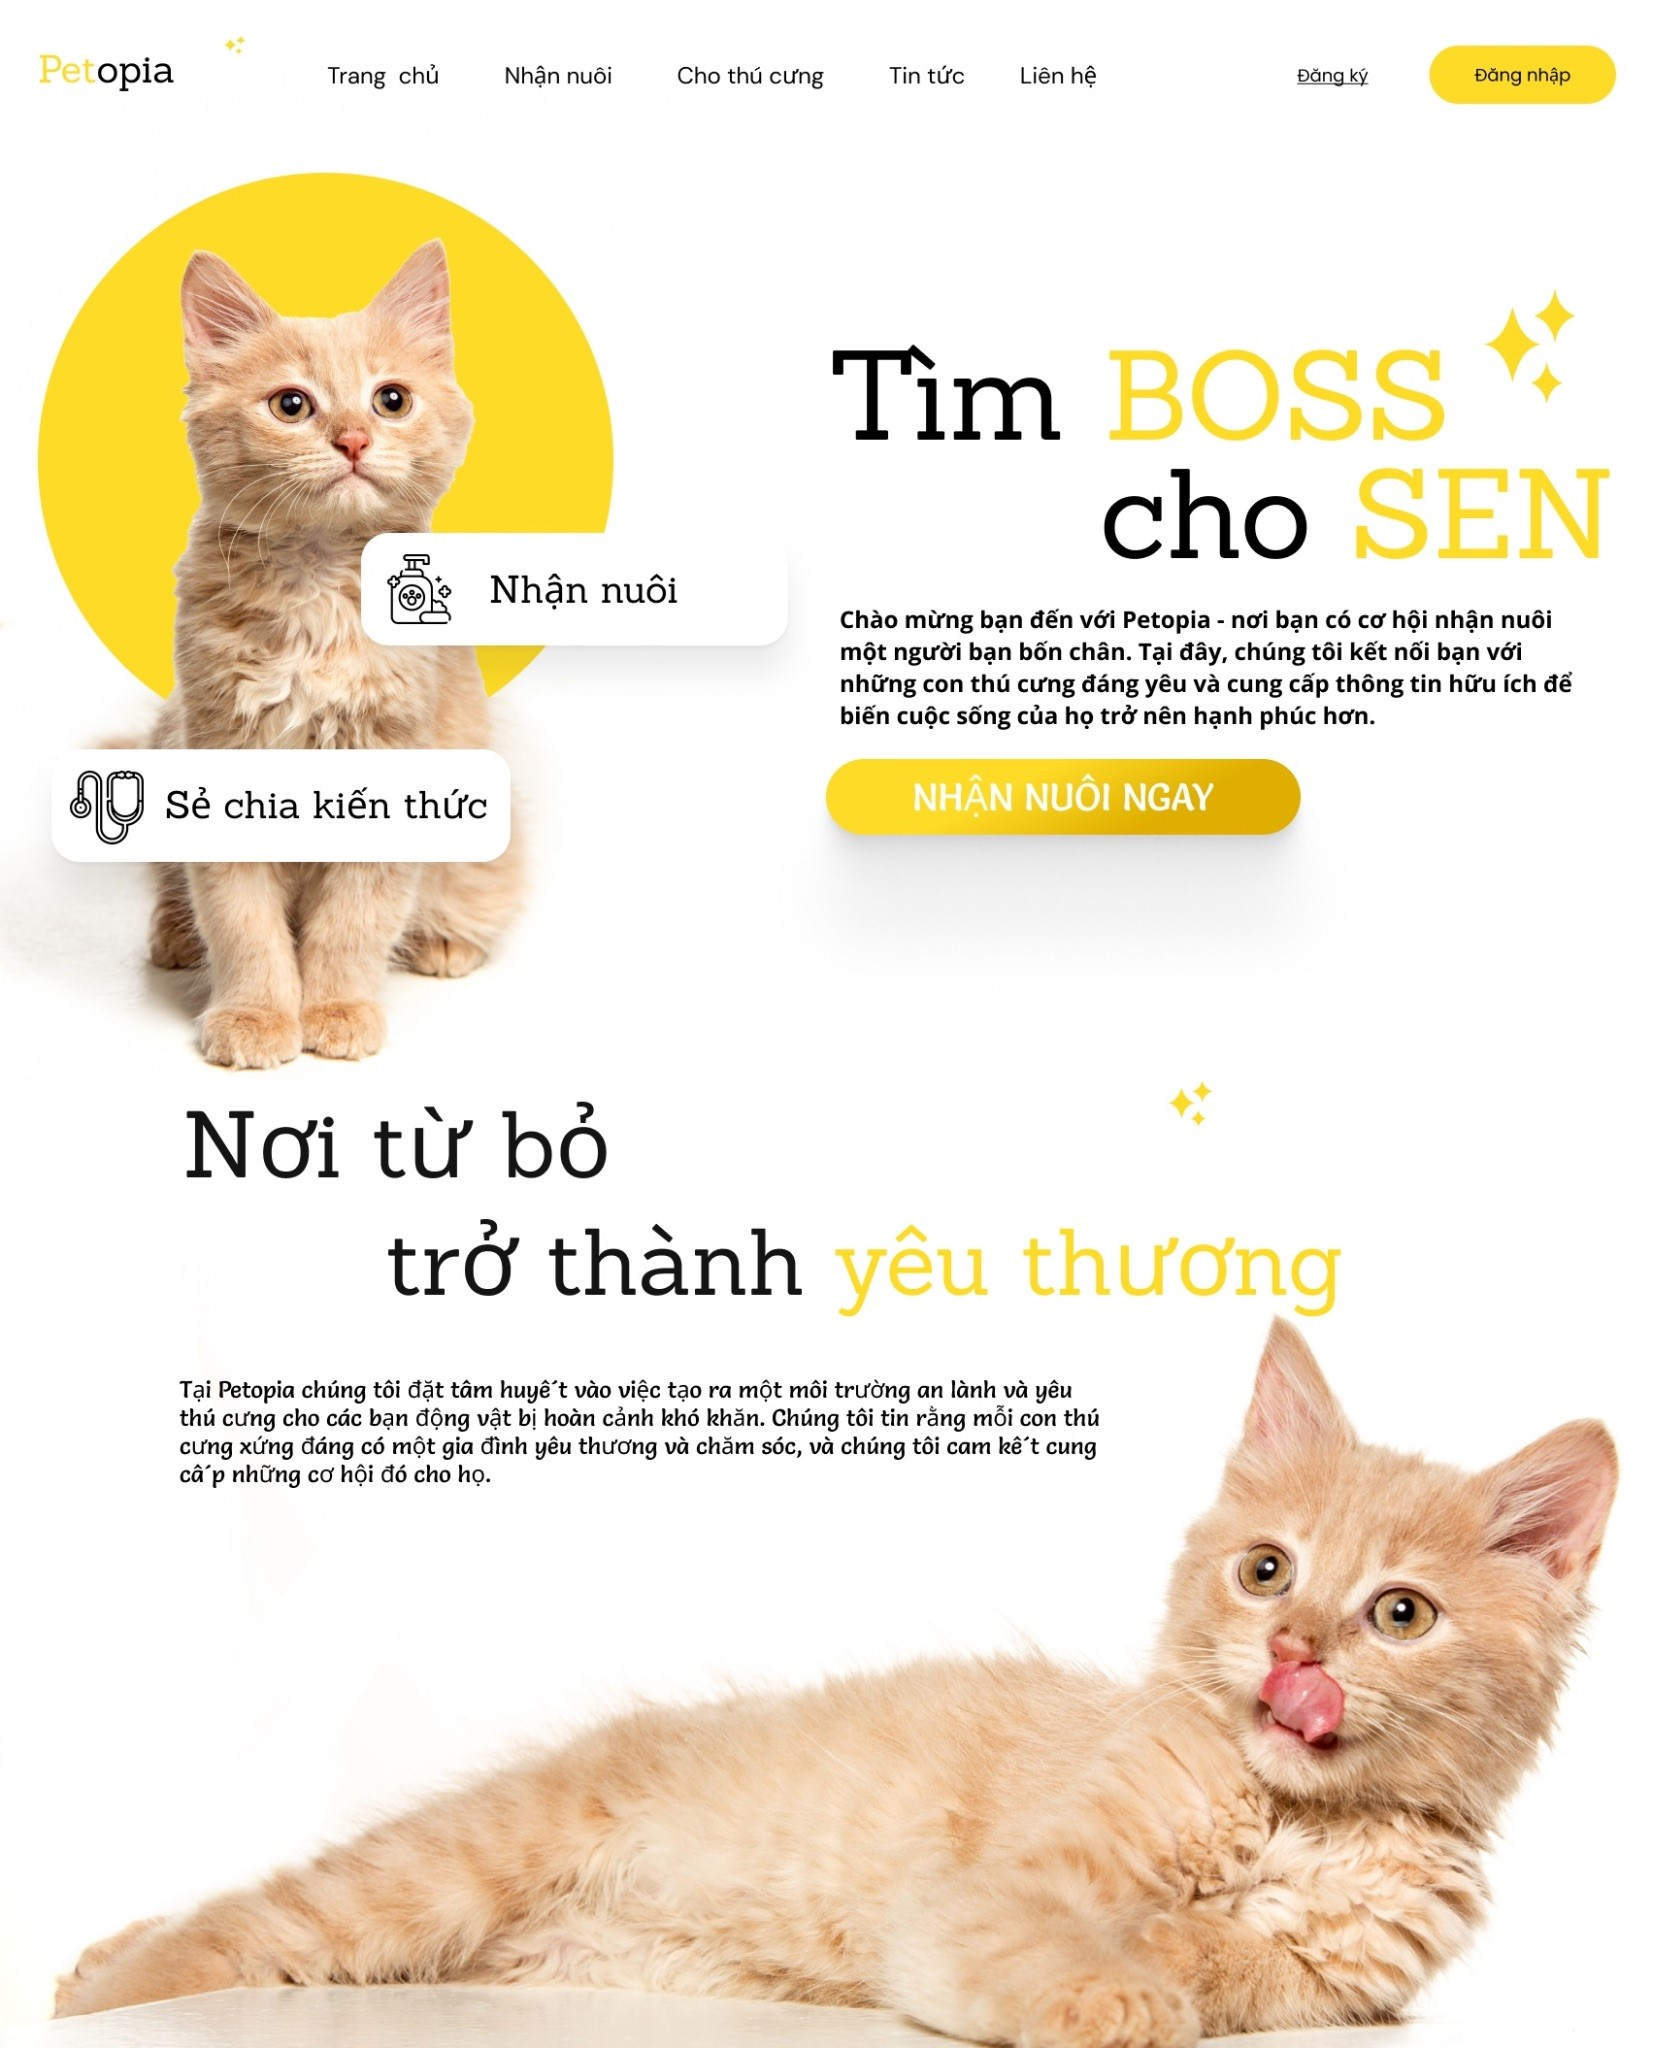
\includegraphics[width=0.8\textwidth]{Figures/home_ui.jpg}
\caption{Homepage of Petopia}
\end{figure}

\subsubsection{Login}

Our homepage's login functionality is designed for simplicity and security, providing a seamless entry into the pet adoption experience. Users can access the login page with a click on the "Đăng nhập" button, where they input their Gmail and password. Error notifications guide users in case of issues, and a convenient register button directs new users to the registration page. For accessibility, users can also log in using their Google account, streamlining the process. A "Forgot Password" option is available for password resets, ensuring a hassle-free and secure experience that accommodates diverse user preferences.

\begin{figure}[H]
    \centering
    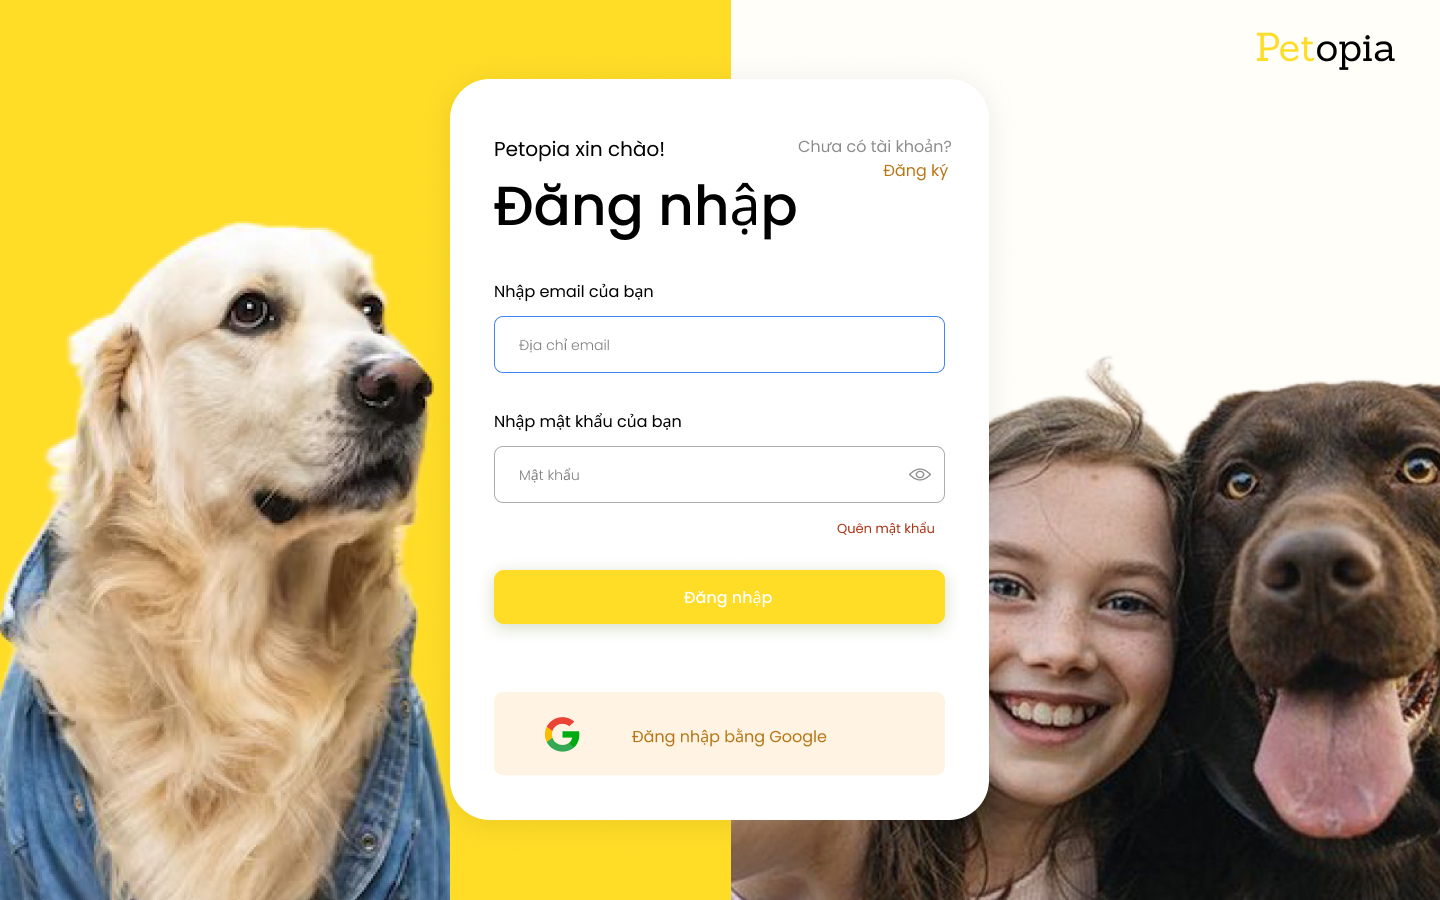
\includegraphics[width=0.8\textwidth]{Figures/login_ui.png}
    \caption{Login form}
\end{figure}

\subsubsection{Register}

The registration process is straightforward, requiring users to input essential information such as first name, last name, Gmail, and password. After clicking "Register," the system verifies the form's completeness and prompts users to check their email for account verification. A verification link enhances security, ensuring authenticity. Clicking the link redirects users to the login page, confirming successful account creation. This two-step process prioritizes security and user-friendly guidance, fostering trust in our platform.

\begin{figure}[H]
    \centering
    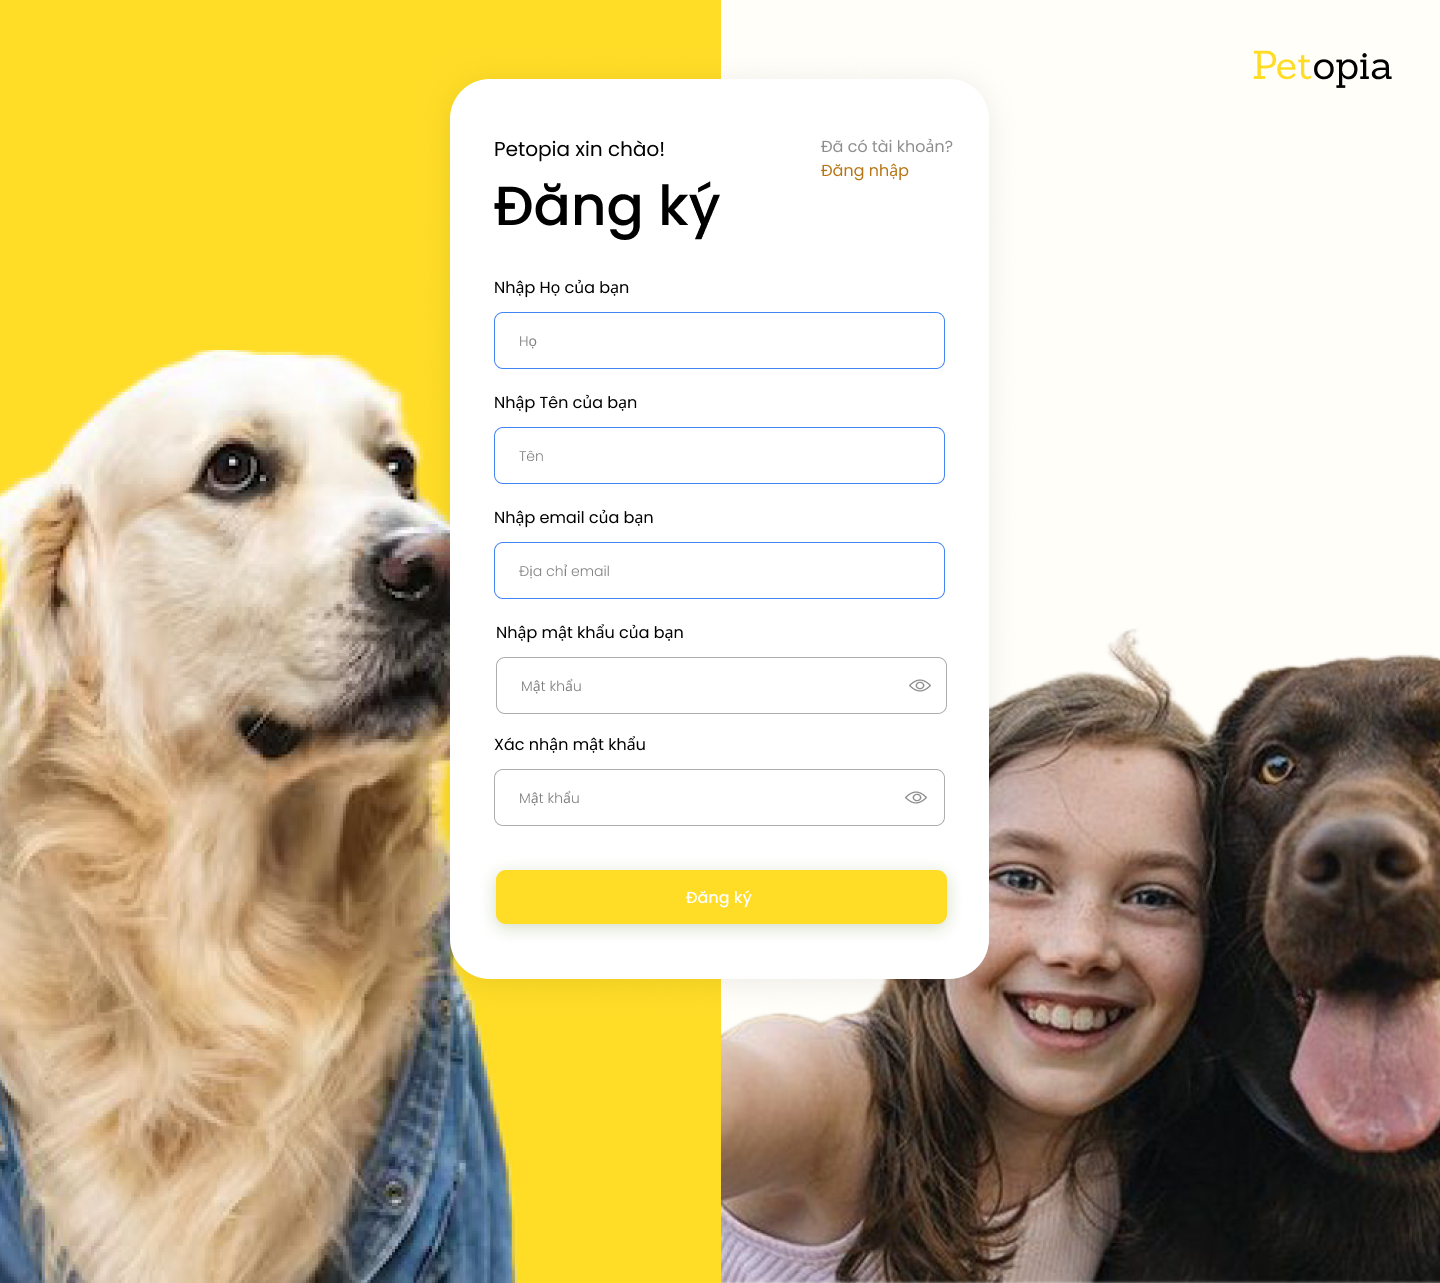
\includegraphics[width=0.5\textwidth]{Figures/register_ui.png}
    \caption{Register form}
\end{figure}

\subsubsection{Search page}

The pet search page is designed for precision and ease. Users can tailor their search with checkboxes for sex, breed, color, size, and vaccination status. A sorting feature arranges results for flexibility. A prominent search bar, and supporting text and image queries, ensure a personalized and efficient experience. Robust filtering, sorting, and versatile search methods aim to provide a user-friendly pet discovery journey on our platform.

\begin{figure}[H]
    \centering
    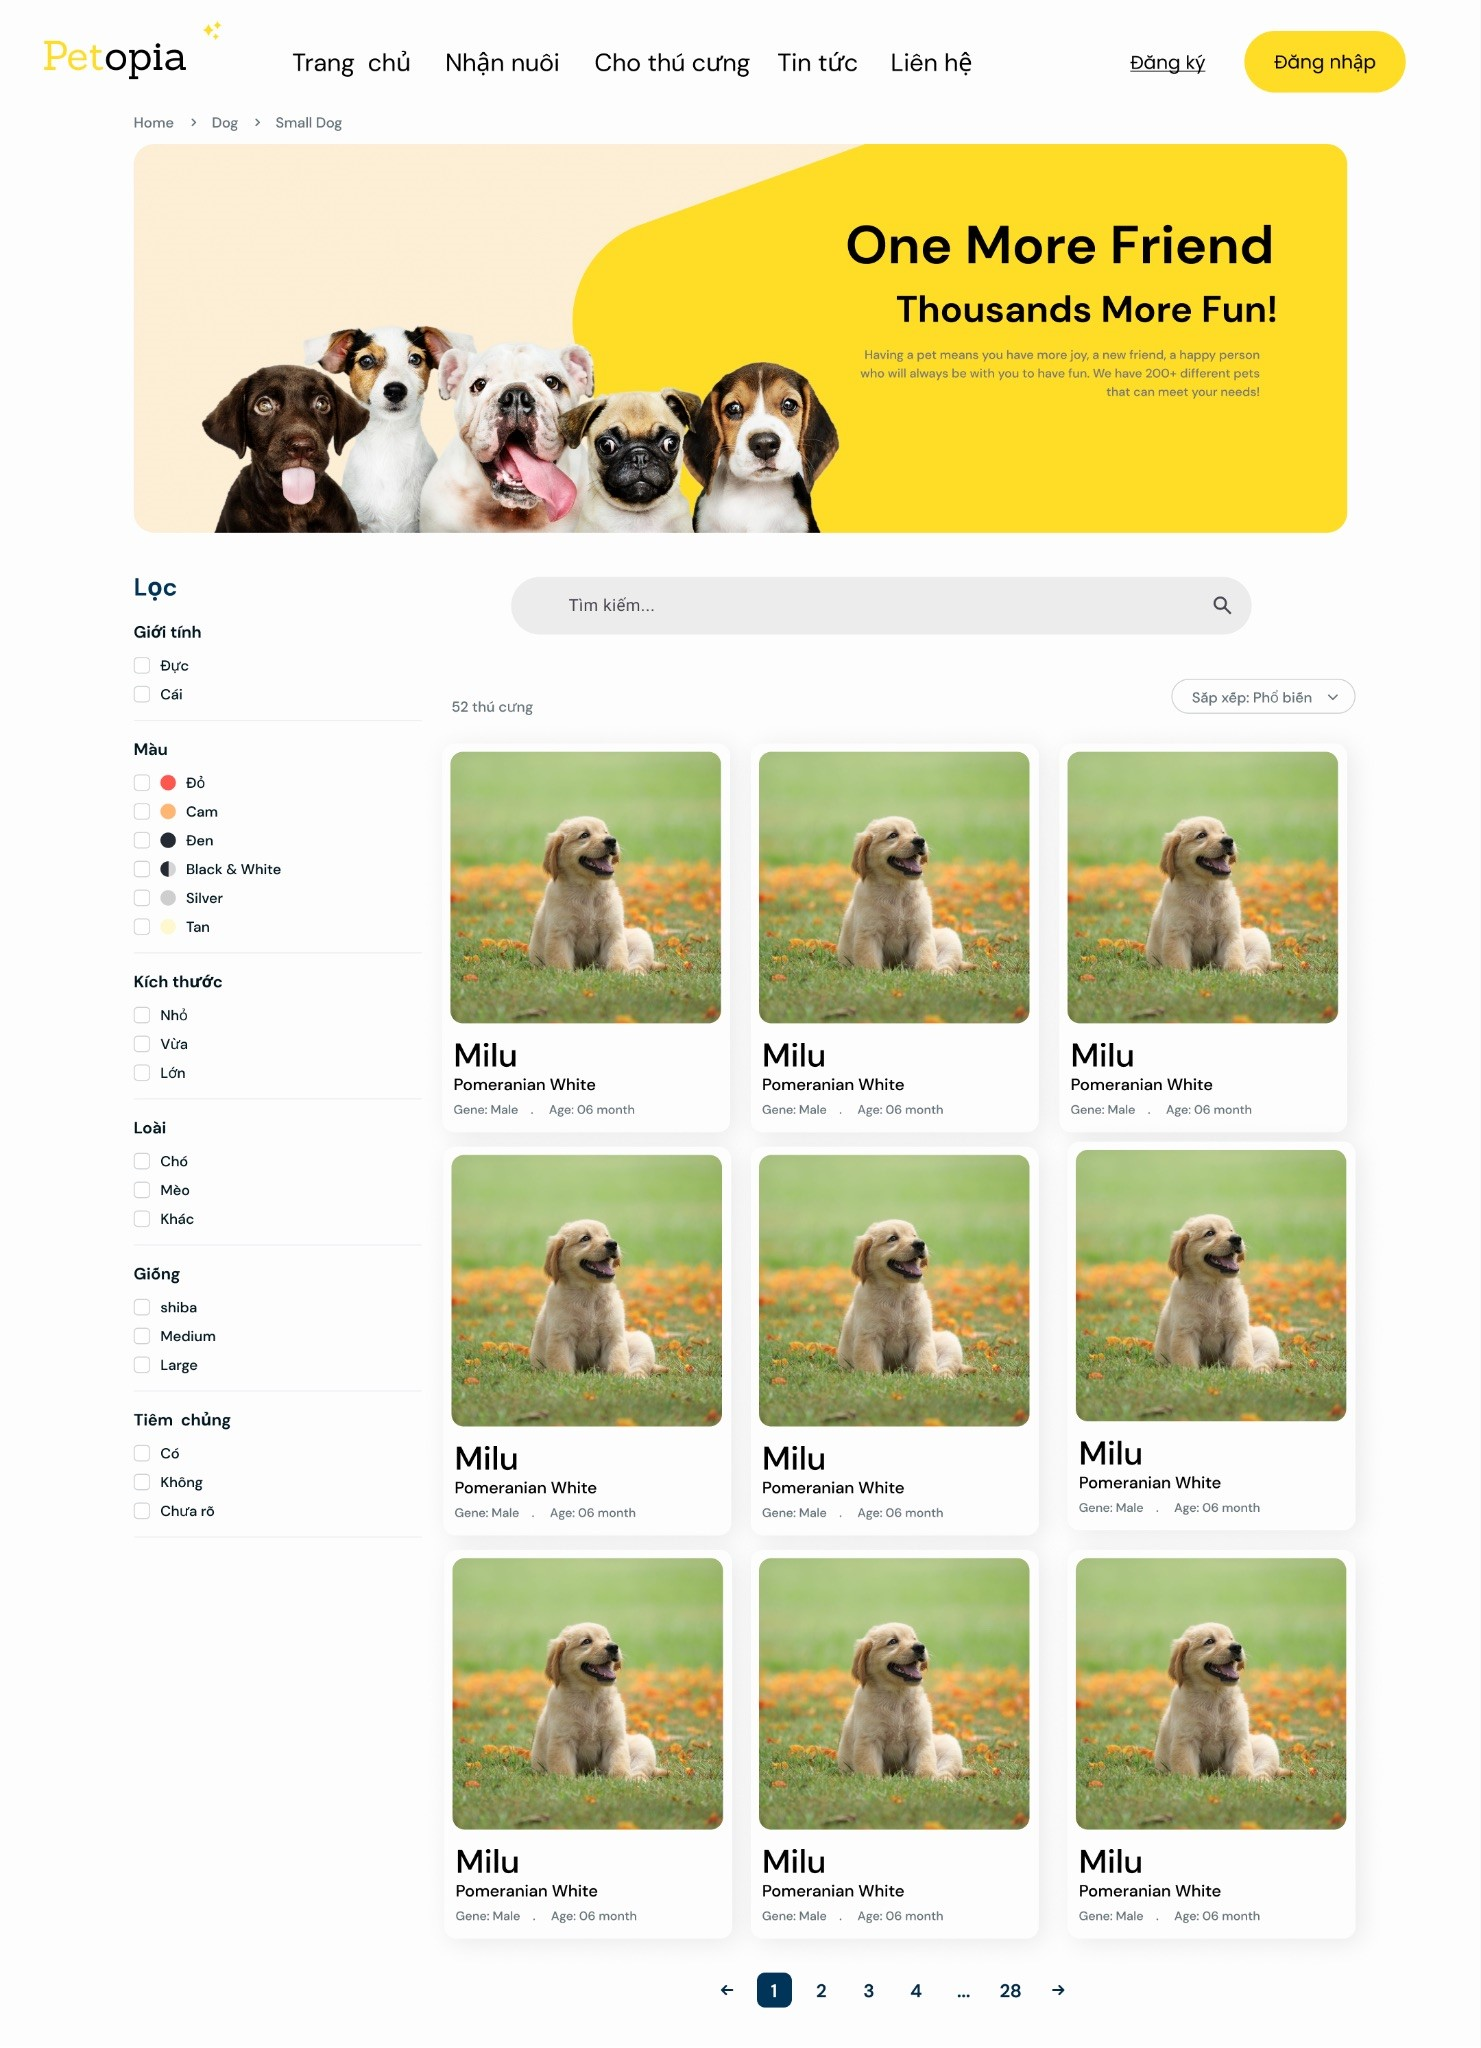
\includegraphics[width=0.8\textwidth]{Figures/search_ui.jpg}
    \caption{Search page for searching desired pet}
\end{figure}


\subsubsection{Pet profile}

The pet page is a comprehensive showcase, providing detailed insights into each pet. Clicking on a pet card redirects users to the dedicated pet profile page, displaying key information such as name, breed, age, and vaccination status. Striking images and a personal description offer a deeper understanding of the pet's personality. A prominent "Adopt" button facilitates the adoption process, dynamically revealing an efficient adoption form upon click. This ensures transparent communication between potential adopters and pet owners.

\begin{figure}[H]
    \centering
    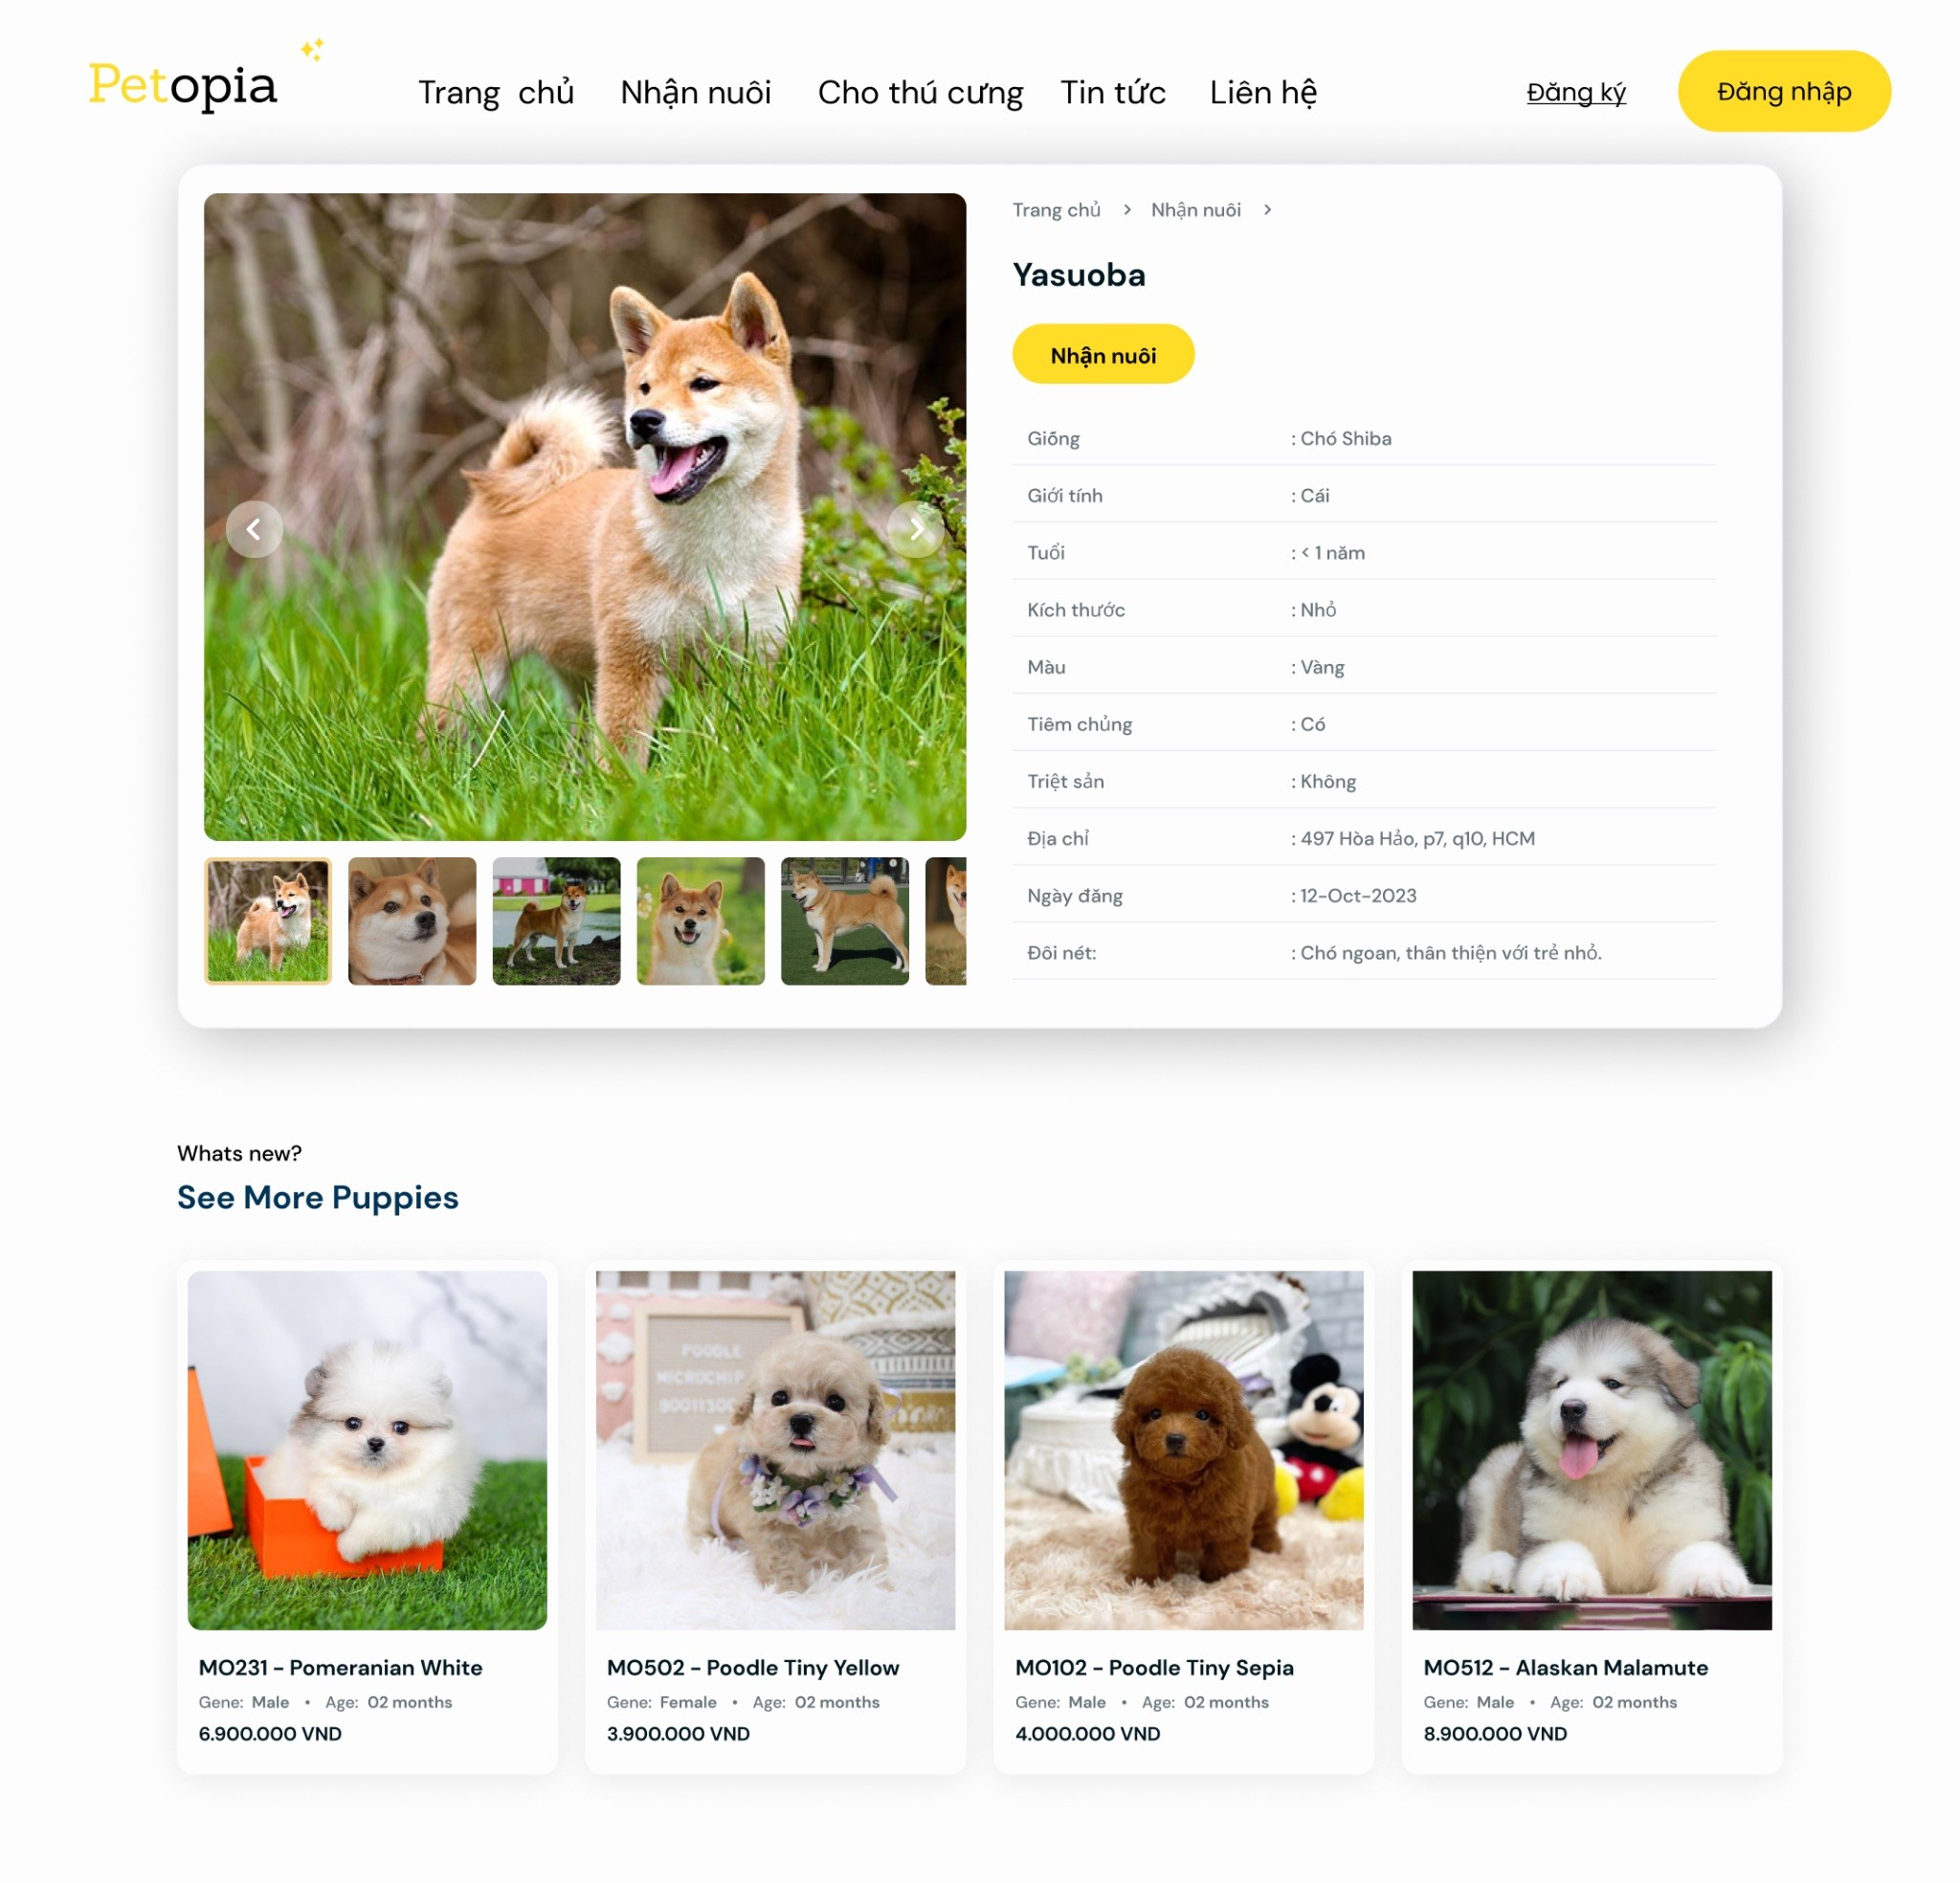
\includegraphics[width=0.8\textwidth]{Figures/pet_detail_ui.jpg}
    \caption{Pet profile page}
\end{figure}

\subsubsection{Create pet profile}

\begin{figure}[H]
    \centering
    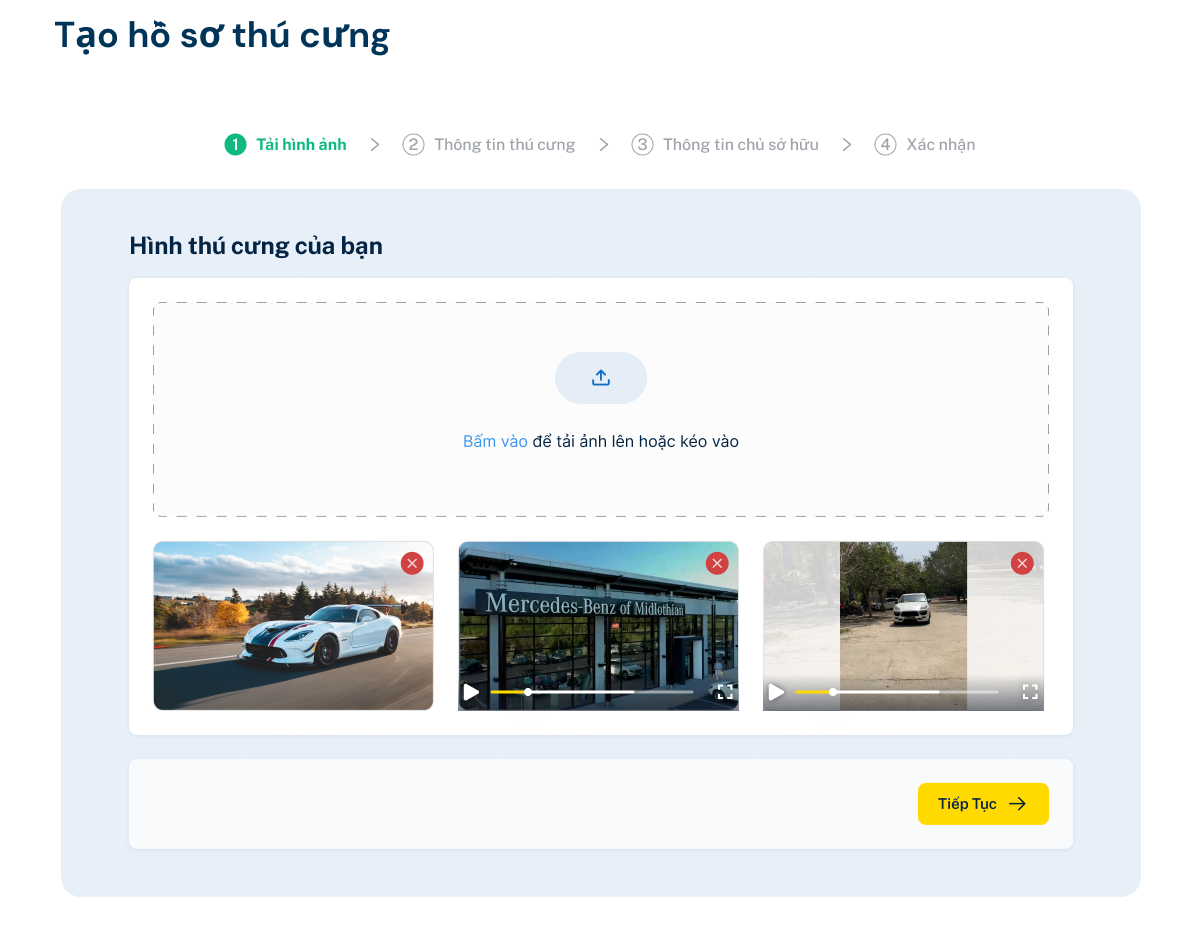
\includegraphics[width=0.7\textwidth]{Figures/img_upload_ui.png}
    \caption{Image upload form}
\end{figure}

\begin{figure}[H]
    \centering
    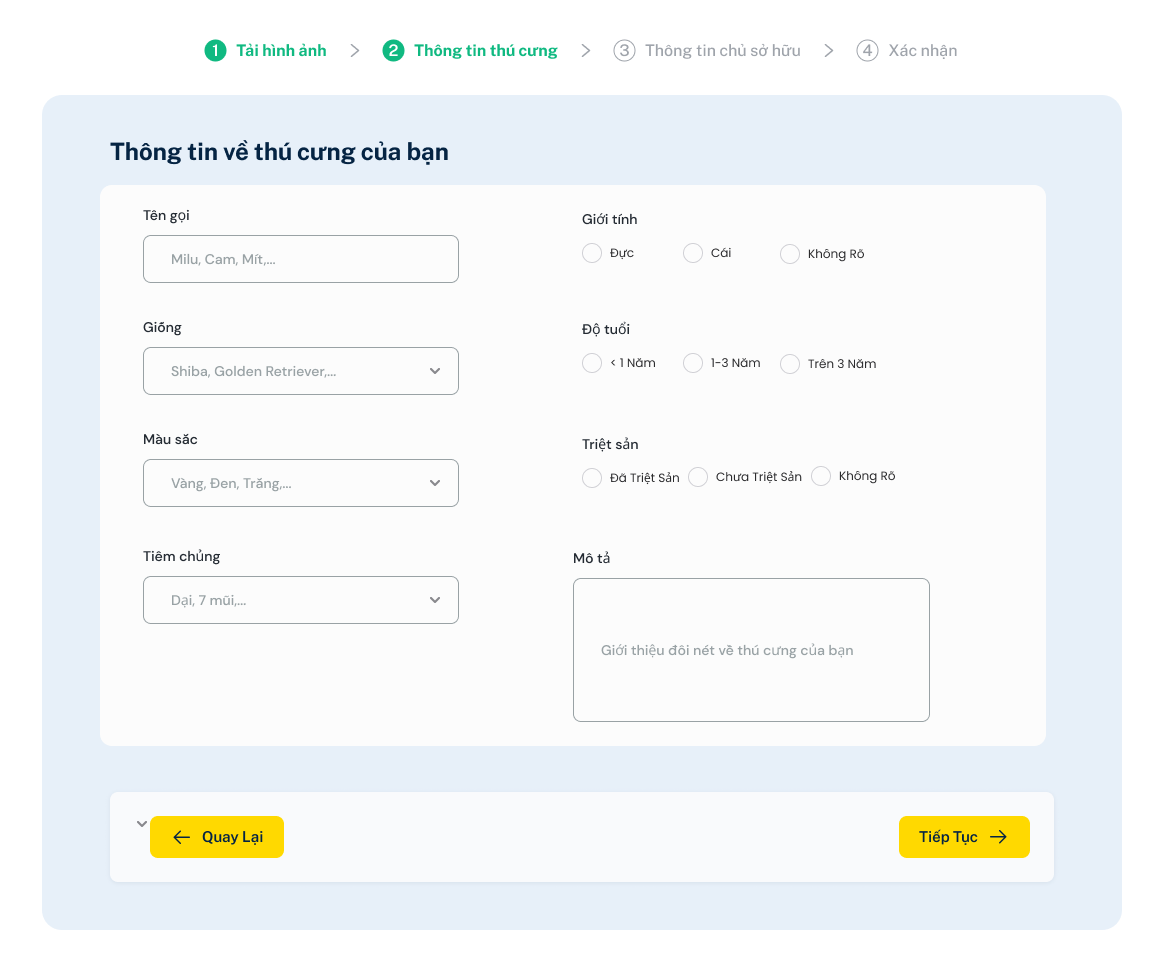
\includegraphics[width=0.7\textwidth]{Figures/pet_input_ui.png}
    \caption{Form for taking user’s pet detail}
\end{figure}

\begin {figure}[H]
\centering
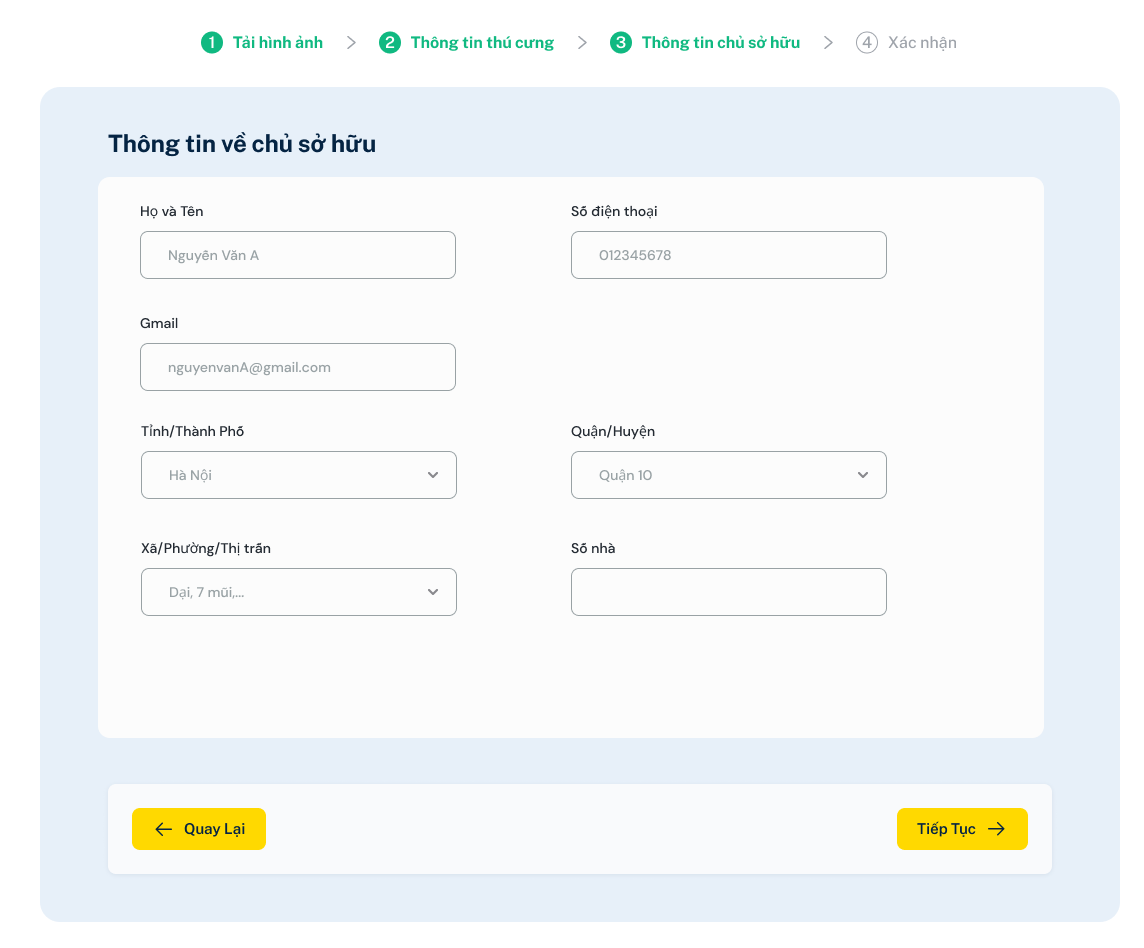
\includegraphics[width=0.7\textwidth]{Figures/user_input_ui.png}
\caption{Create pet profile page}
\end{figure}

\begin {figure}[H]
\centering
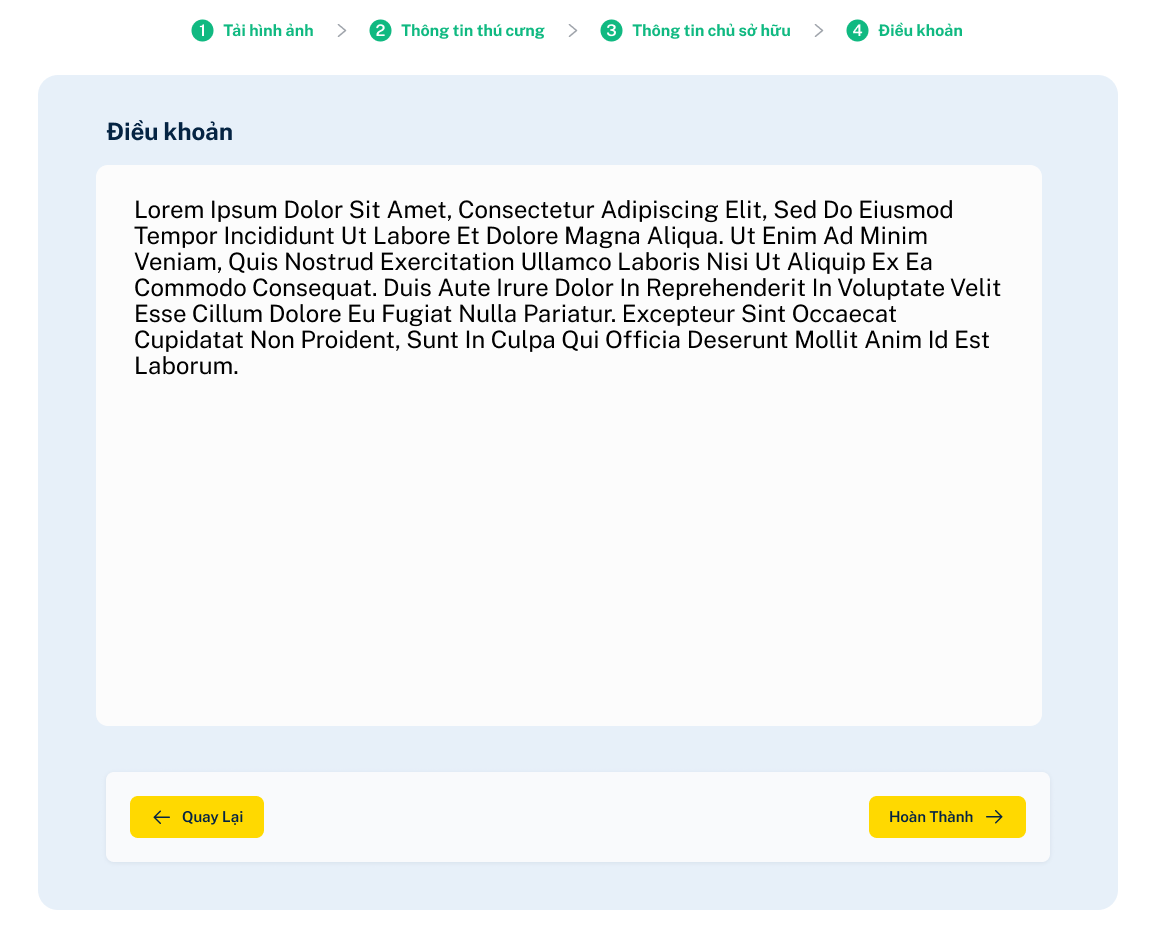
\includegraphics[width=0.7\textwidth]{Figures/term_ui.png}
\caption{Pet profile page}
\end{figure}

Creating a pet profile on our platform is user-friendly and efficient. Users start by providing a pet figure (Figure 43), processed by our AI to autofill certain fields like breed and color. Clicking "Continue" guides users through a pet form (Figure 44) for additional details. Afterward, an owner form (Figure 45) captures essential information, followed by a review of Terms and Services (Figure 46) before clicking "Finish" to complete the profile. This structured process, aided by AI in the initial steps, ensures accuracy and a seamless user experience.

\subsubsection{User profile}

\begin{figure}[H]
    \centering
    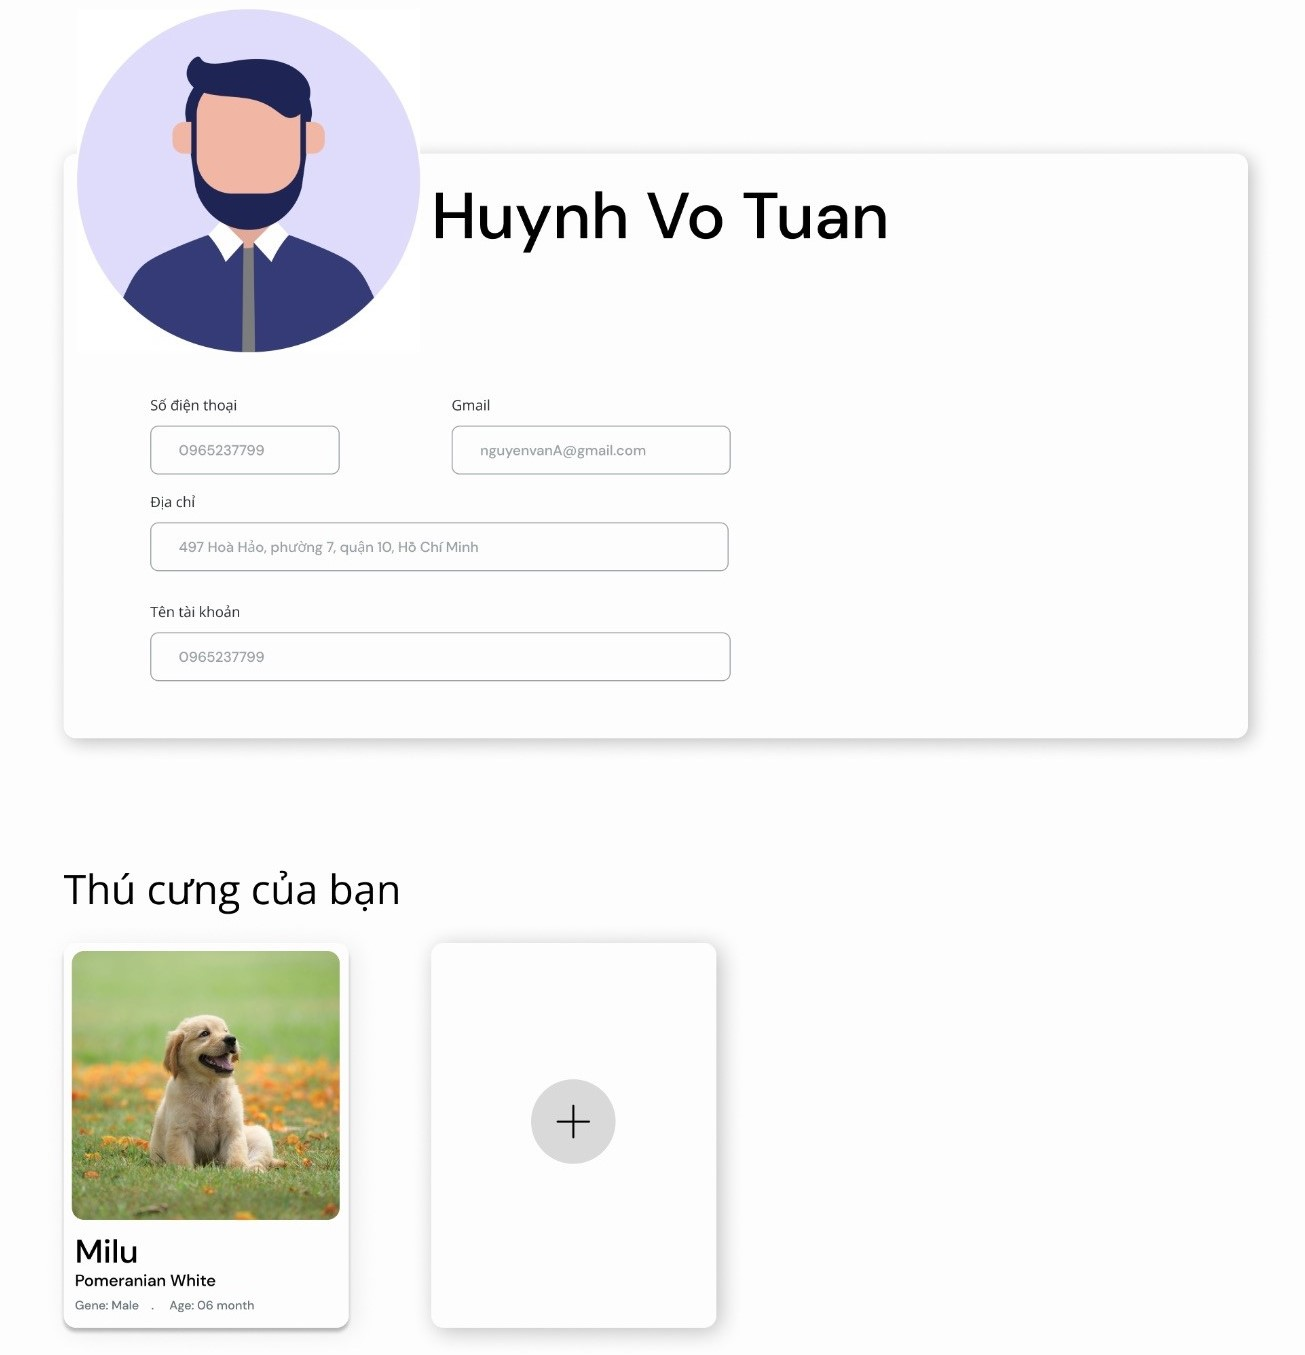
\includegraphics[width=0.7\textwidth]{Figures/user_profile_ui.jpg}
    \caption{User profile page}
\end{figure}


The user profile page serves as a centralized hub for managing and personalizing information. It prominently displays the user's avatar, name, address, Gmail, and phone number, allowing easy editing for up-to-date details. The page also showcases pet profiles, encouraging users to create new ones with a streamlined process. This intuitive design ensures a seamless and enjoyable experience for users to manage personal information and engage with our platform's pet adoption features.

\subsubsection{Blog homepage}
\begin{figure}[H]
    \centering
    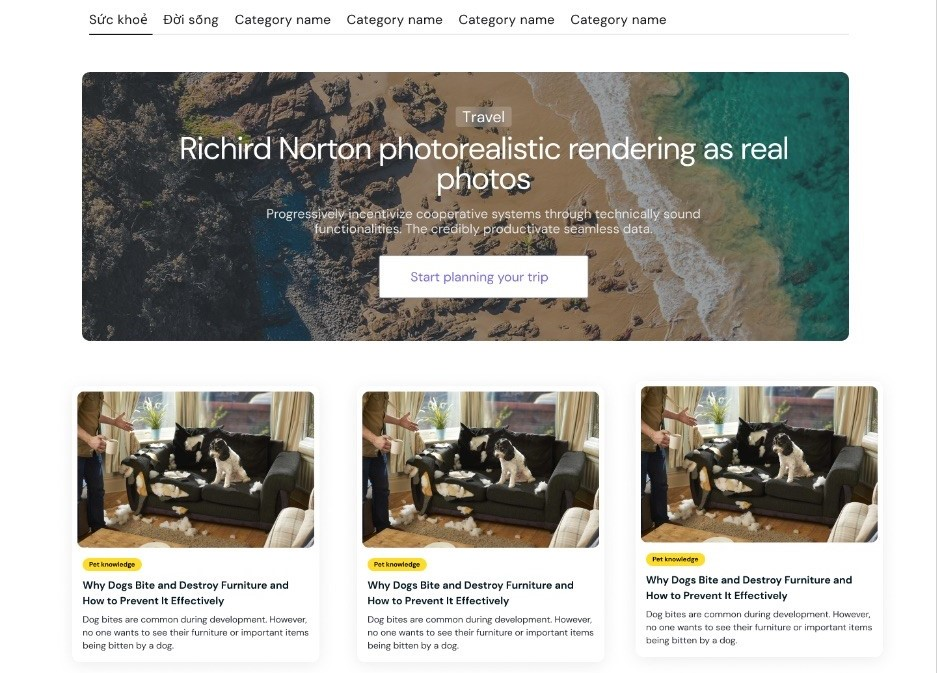
\includegraphics[width=0.8\textwidth]{Figures/blog_ui.jpg}
    \caption{Blog homepage}
\end{figure}

The blog homepage offers a curated space with various categories for users to explore diverse content. Clicking a category dynamically displays relevant blogs, ensuring a targeted reading experience. Selecting a specific blog seamlessly redirects users to the dedicated blog page for detailed exploration. Integrated ads support the platform without disrupting the user experience, contributing to the sustainability of our blog platform.

\subsubsection{Blog page}

\begin{figure}[H]
    \centering
    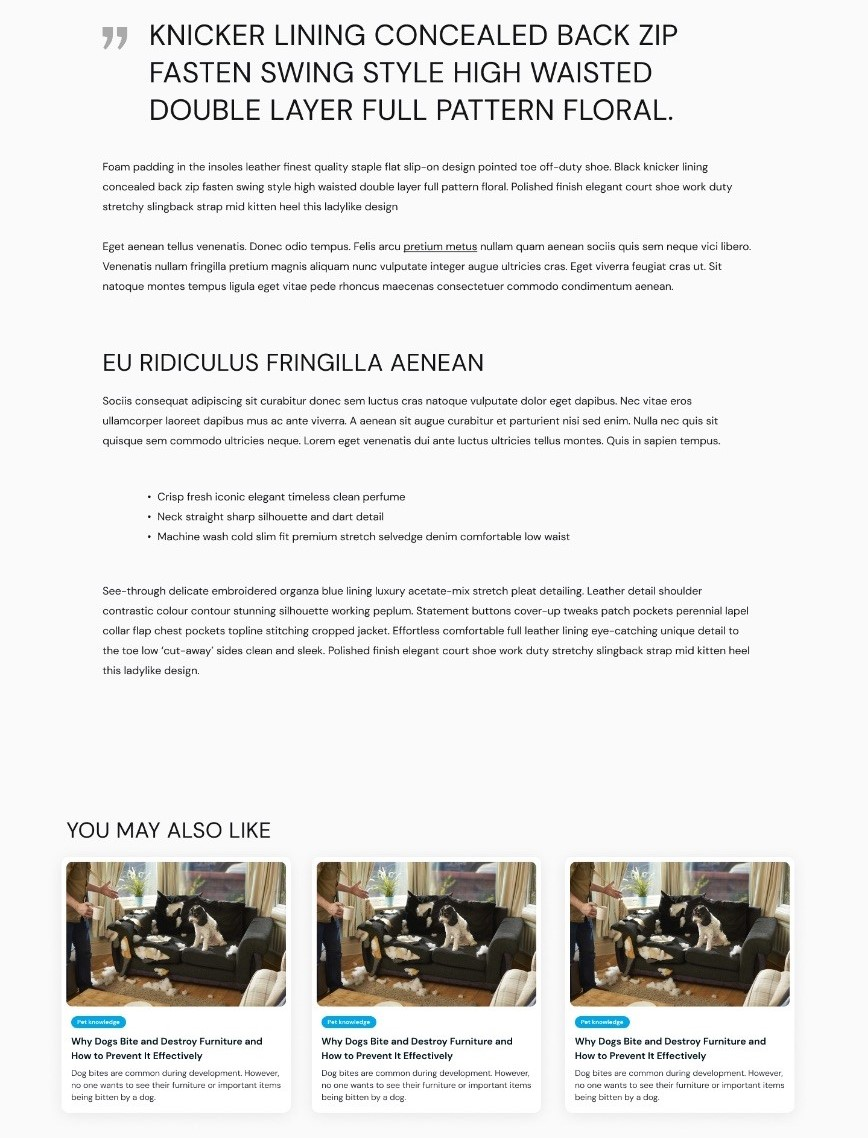
\includegraphics[width=0.8\textwidth]{Figures/blog_page_ui.jpg}
    \caption{Blog page}
\end{figure}

The blog page ensures a rich and interactive reading experience, allowing users to delve into detailed blog posts. Metrics like view count indicate popularity. Users can easily share content on social channels, fostering community engagement. A relevant section suggests related blogs, encouraging users to explore aligned topics for an enhanced and curated experience.

\subsection{Back office}

\begin{figure}[H]
    \centering
    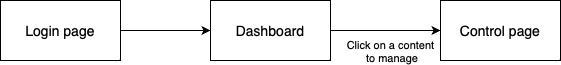
\includegraphics[width=0.8\textwidth]{Figures/wireframe_bo.png}
    \caption{Wireframe for Back office}
\end{figure}

\subsubsection{Login}

\begin{figure}[H]
    \centering
    
\includegraphics[width=0.8\textwidth]{Figures/login_bo_ui.png}
    \caption{Login page for admins}
\end{figure}

The login page requires administrators to input their username and password in the designated fields. Login using Google is not available; only the provided account credentials can be used. Upon correct input, administrators are directed to the dashboard.

\subsubsection{Dashboard}

\begin{figure}[H]
    \centering
    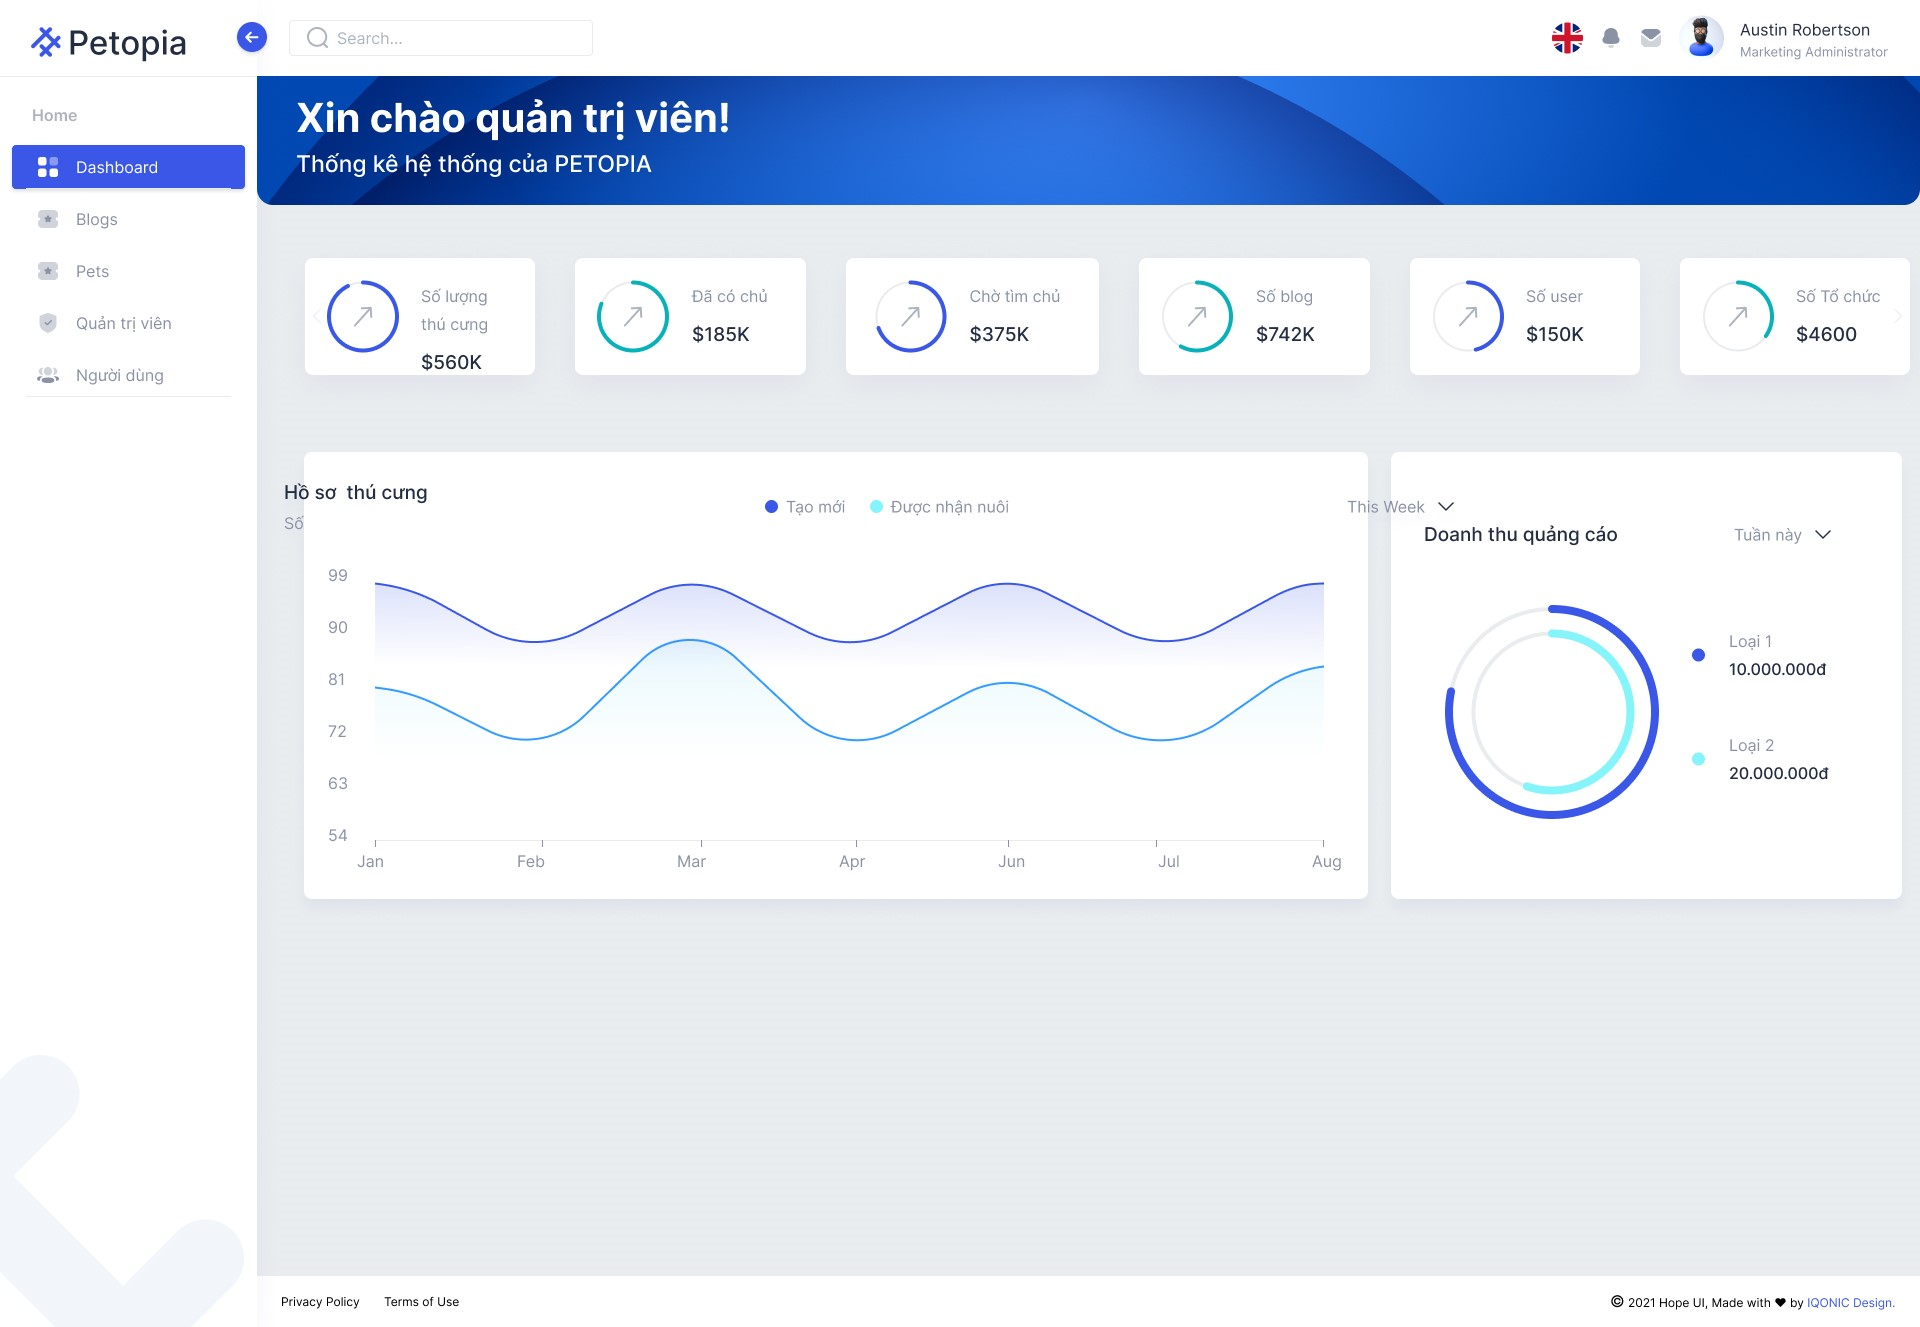
\includegraphics[width=0.8\textwidth]{Figures/dashboard_ui.jpg}
    \caption{Dashboard to show reports and statistics}
\end{figure}

The dashboard page provides administrators with comprehensive insights into the Petopia website. It displays key metrics such as the number of visitors, pets, blogs, and users. To enhance visualization, graphical representations accompany these statistics, offering a clear and dynamic overview of the platform's performance. This feature allows administrators to efficiently monitor and analyze the website's vital statistics at a glance.

\subsubsection{Control page}

The control page empowers administrators to manage specific data types, including users, blogs, and pets. Administrators can access records, apply filters for efficient navigation, edit fields, enable or disable records, and delete them as needed. This functionality provides administrators with a versatile and centralized tool for comprehensive control and customization of various data records on the platform.

\begin {figure}[H]
\centering
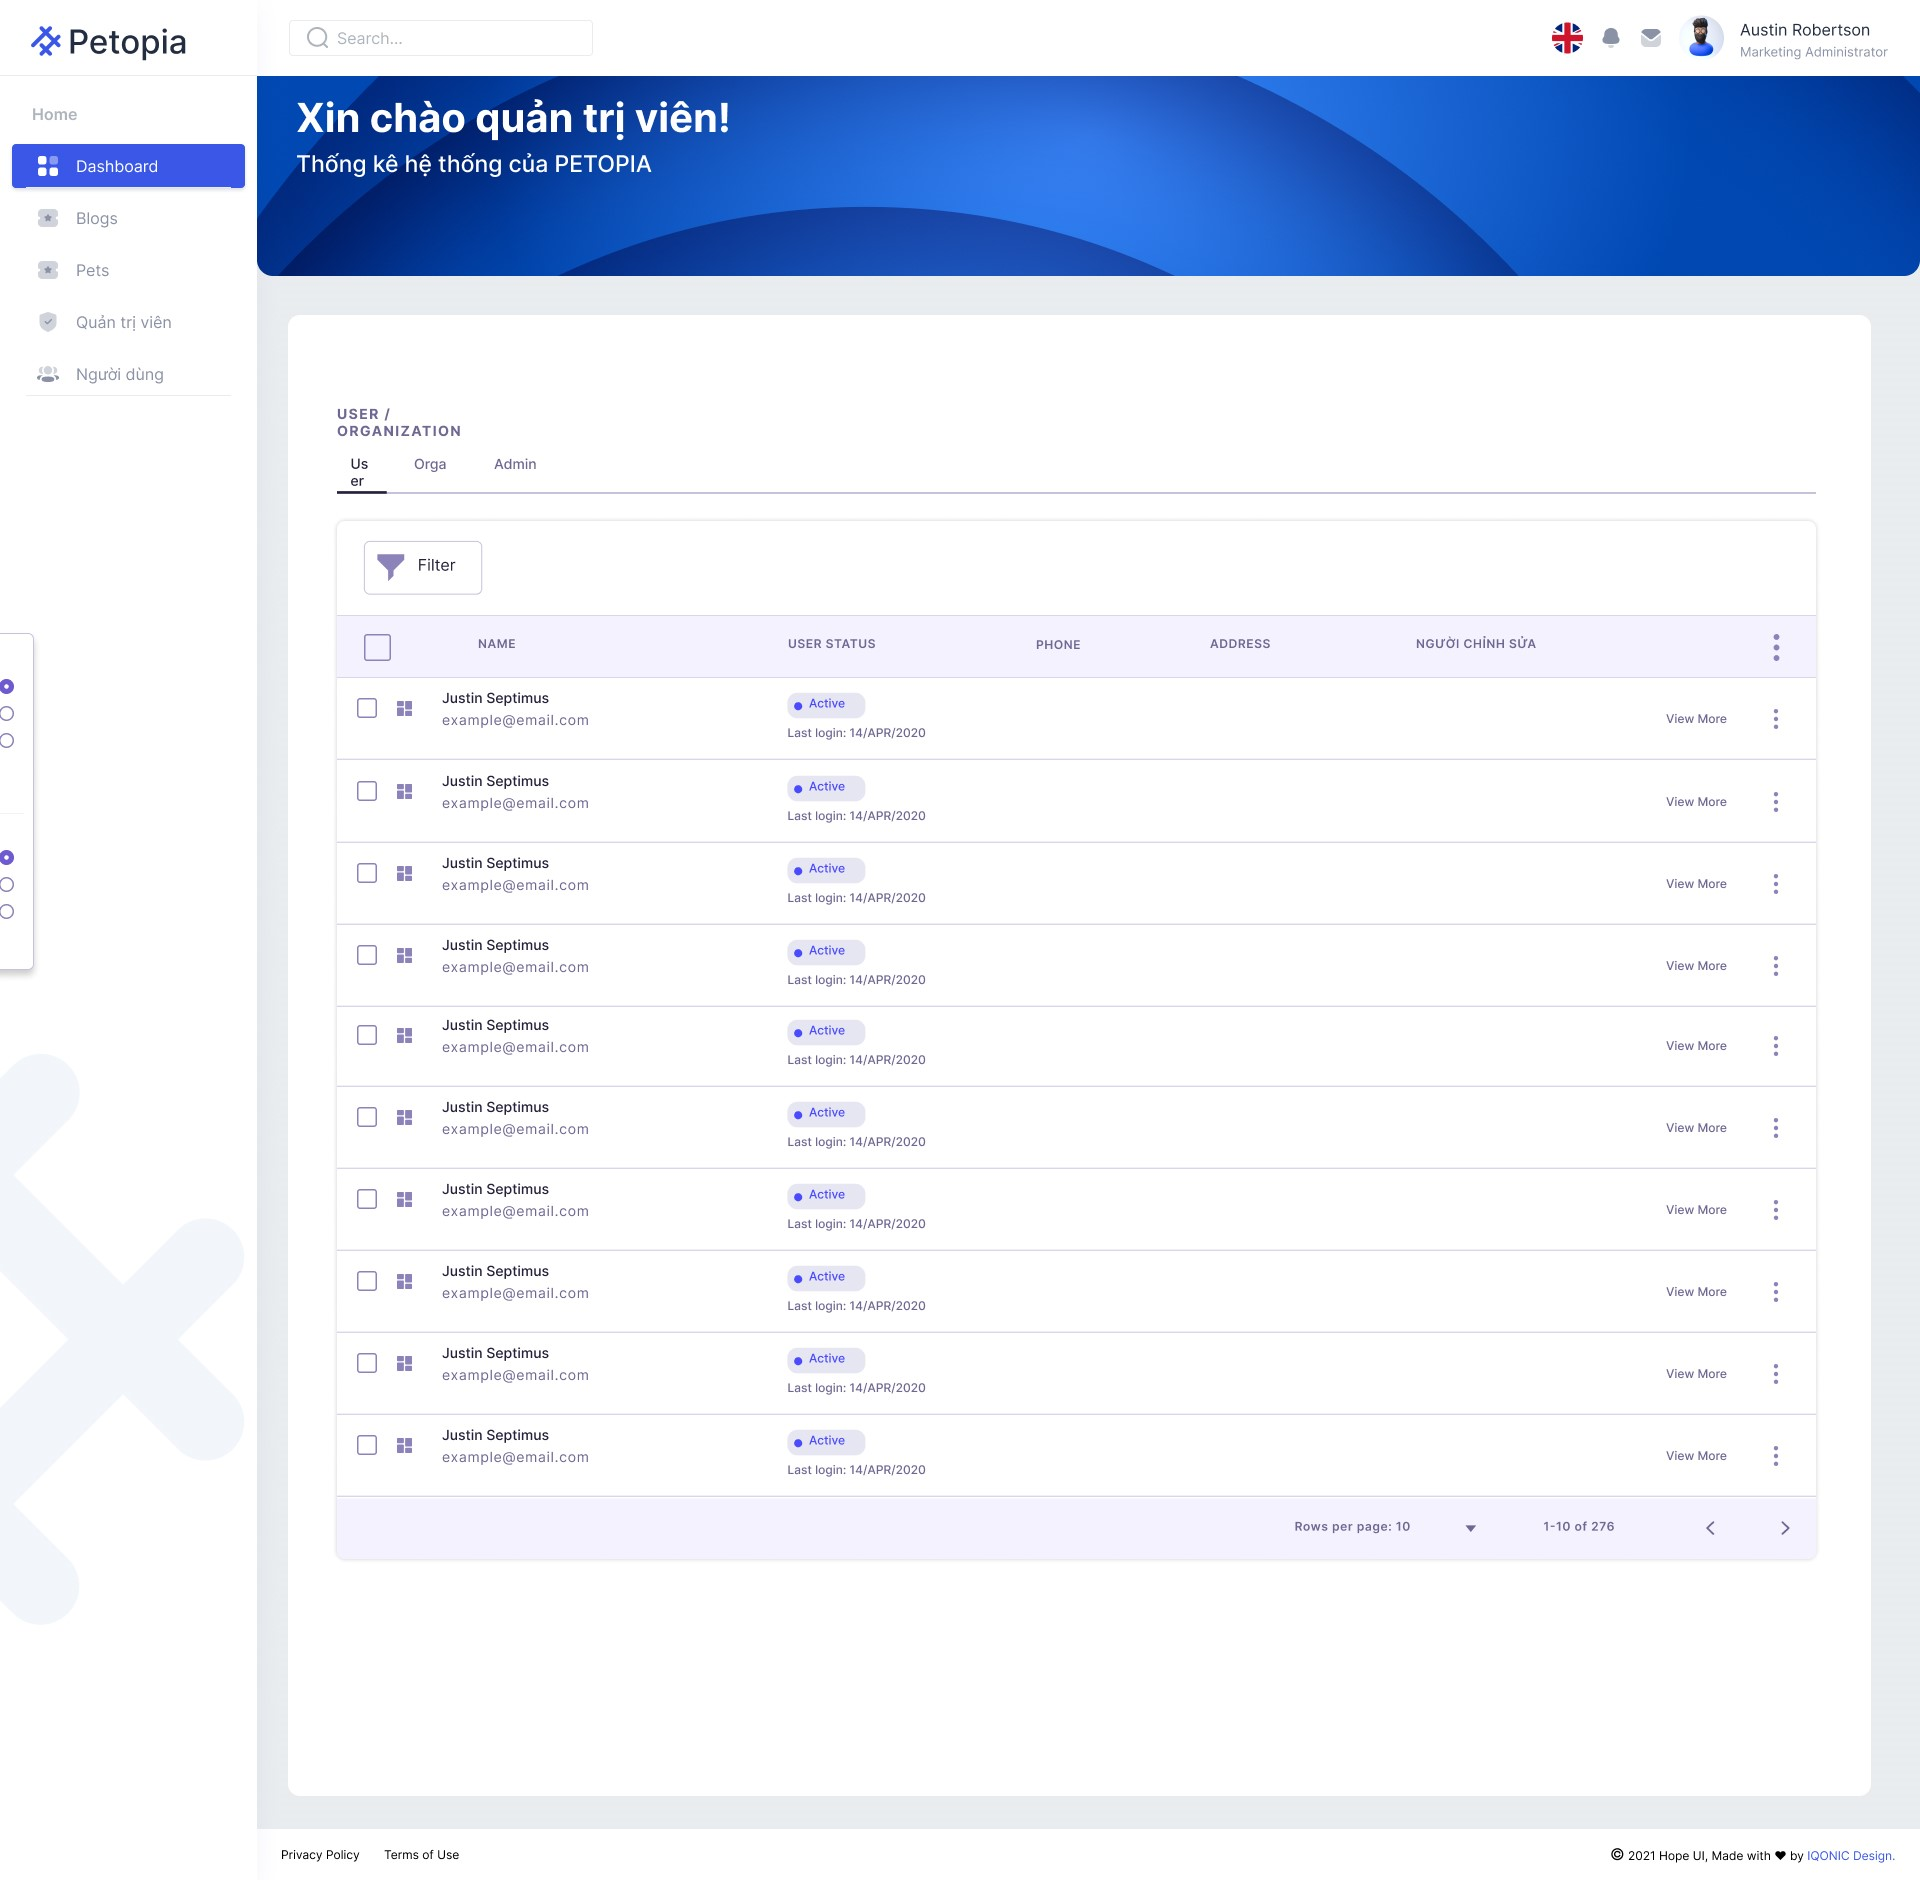
\includegraphics[width=0.8\textwidth]{Figures/control_bo_ui.jpg}
\caption{Control page for managing data records}
\end{figure}

\section{Database design}

\subsection{Conceptual design}

The conceptual design phase of the project is a pivotal stage in the development lifecycle, focused on establishing a comprehensive understanding of the system's structure and relationships.


In \emph{Figure 54}, the main entities and attributes are presented, and
some non-key attributes and entities are excluded to enhance
visualization and maintain a clear focus on the primary components
shaping the system. There are several 3-way relationships presented in
the figure, involving two optional entities linked to a mandatory one,
the presence of the mandatory entity is contingent upon the existence
and participation of the other two entities. Simply put, the mandatory
entity only comes into existence when the other two entities are present
and actively engaged in the relationship.

\begin{figure}[H]
    \centering
    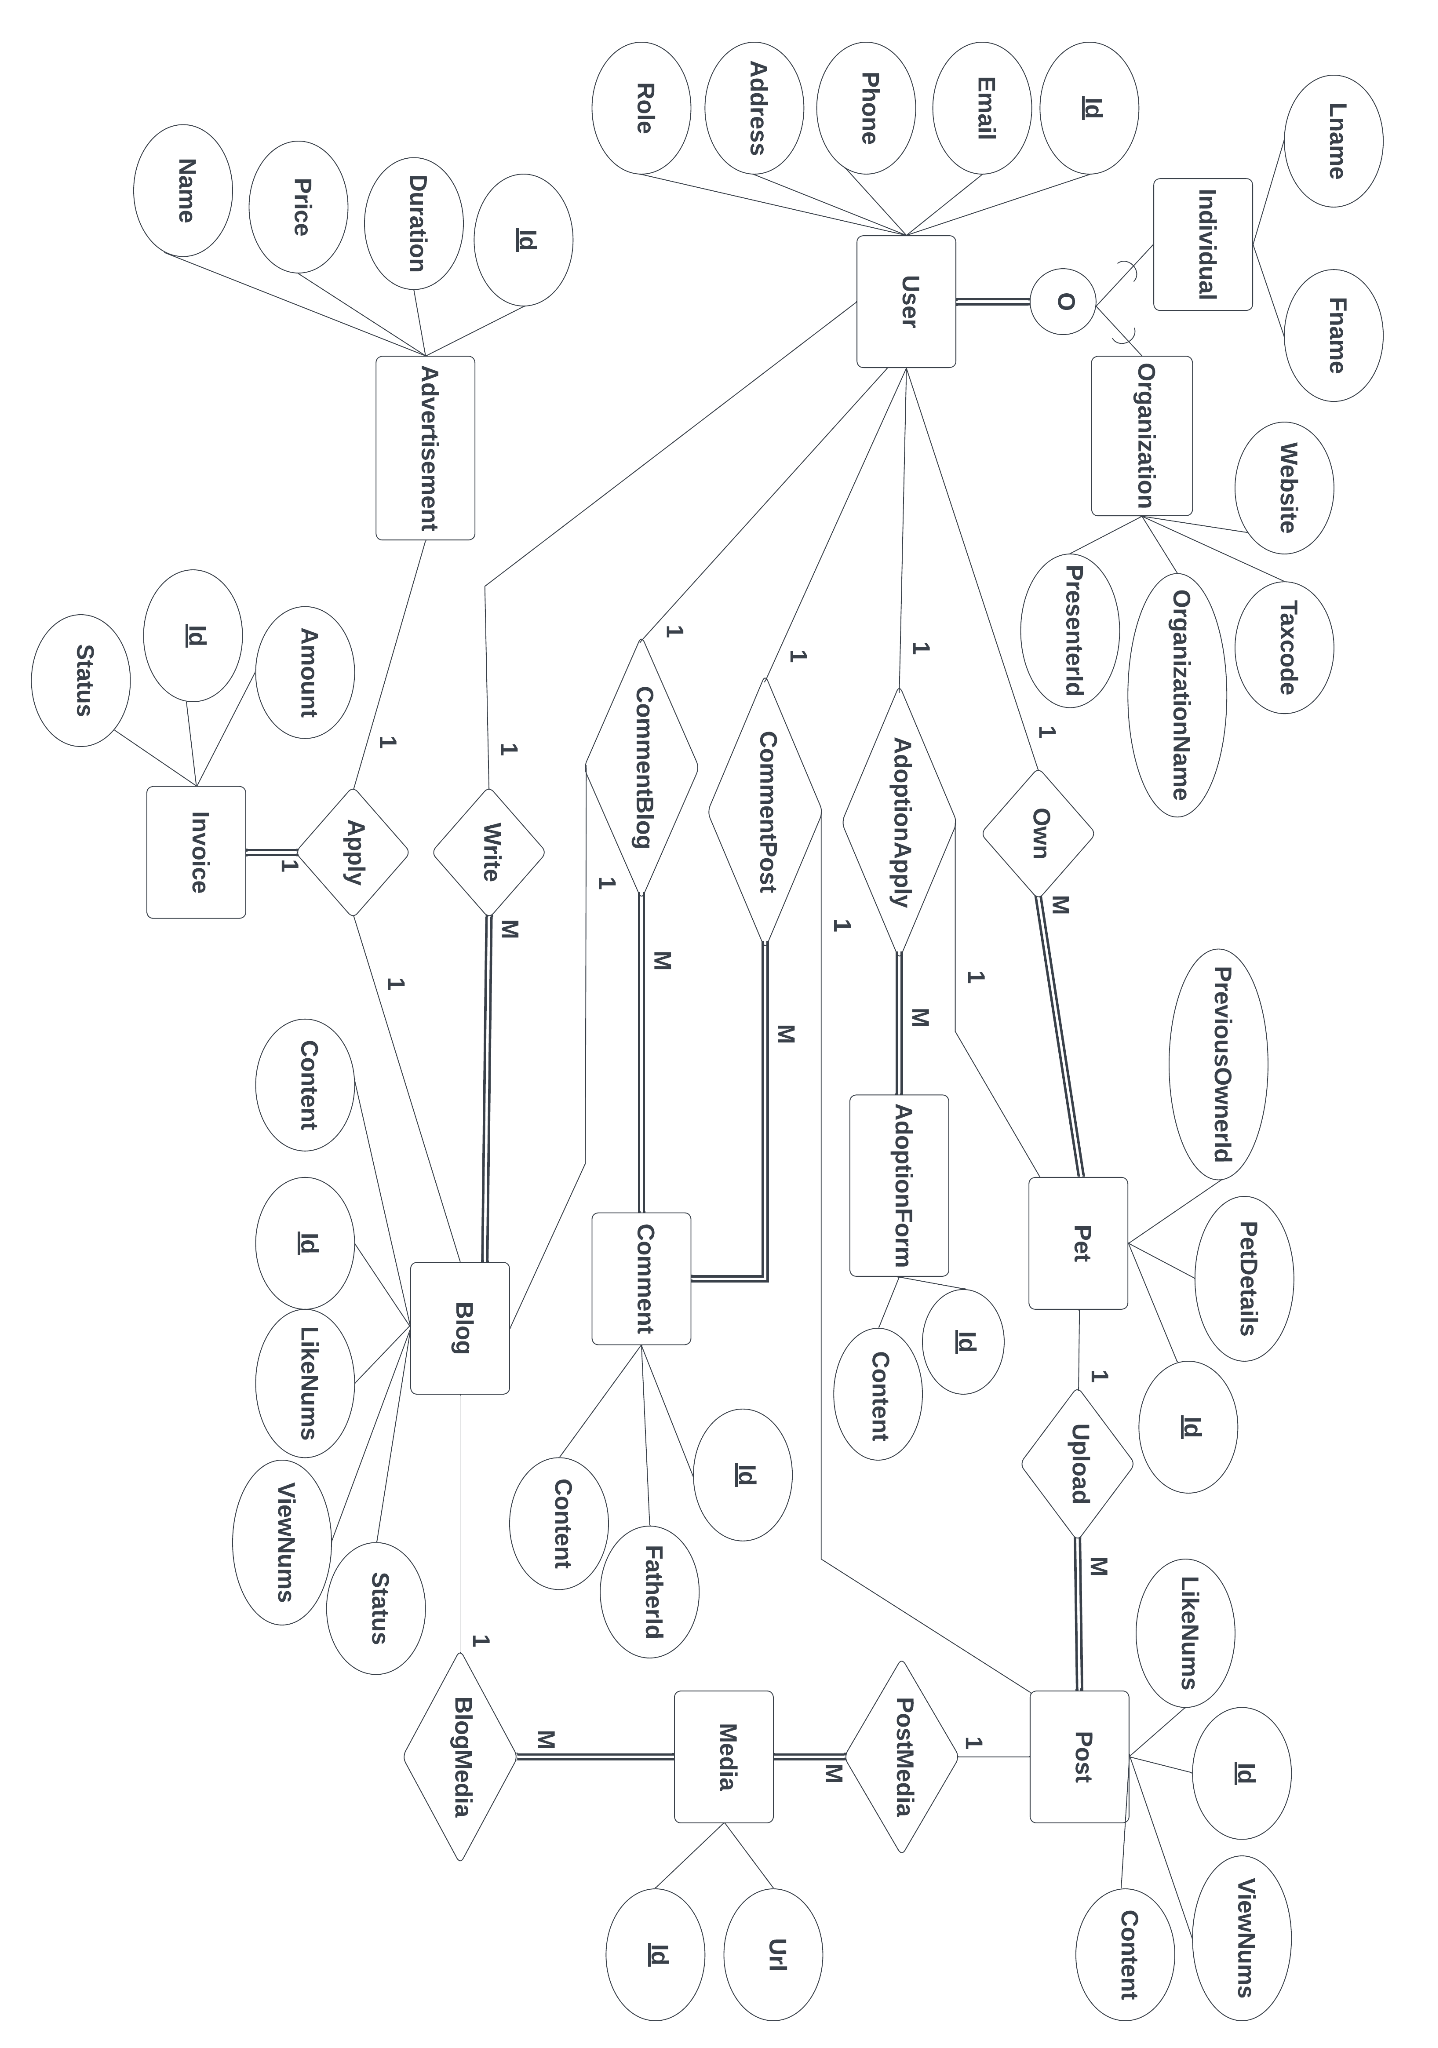
\includegraphics[width=0.8\textwidth]{Figures/erd.png}
    \caption{Entity-Relationship diagram}
\end{figure}
\clearpage

\subsection{Relational Design}

In the relational design phase, we use the relational mapping approach
to translate the abstract concepts from the Entity-Relationship Diagram
(ERD) into a concrete relational schema. Through the mapping process,
each entity, along with its attributes and relationships, is
systematically transformed into tables with defined fields and
corresponding constraints in \emph{Figure 55}.

\begin {figure}[H]
\centering
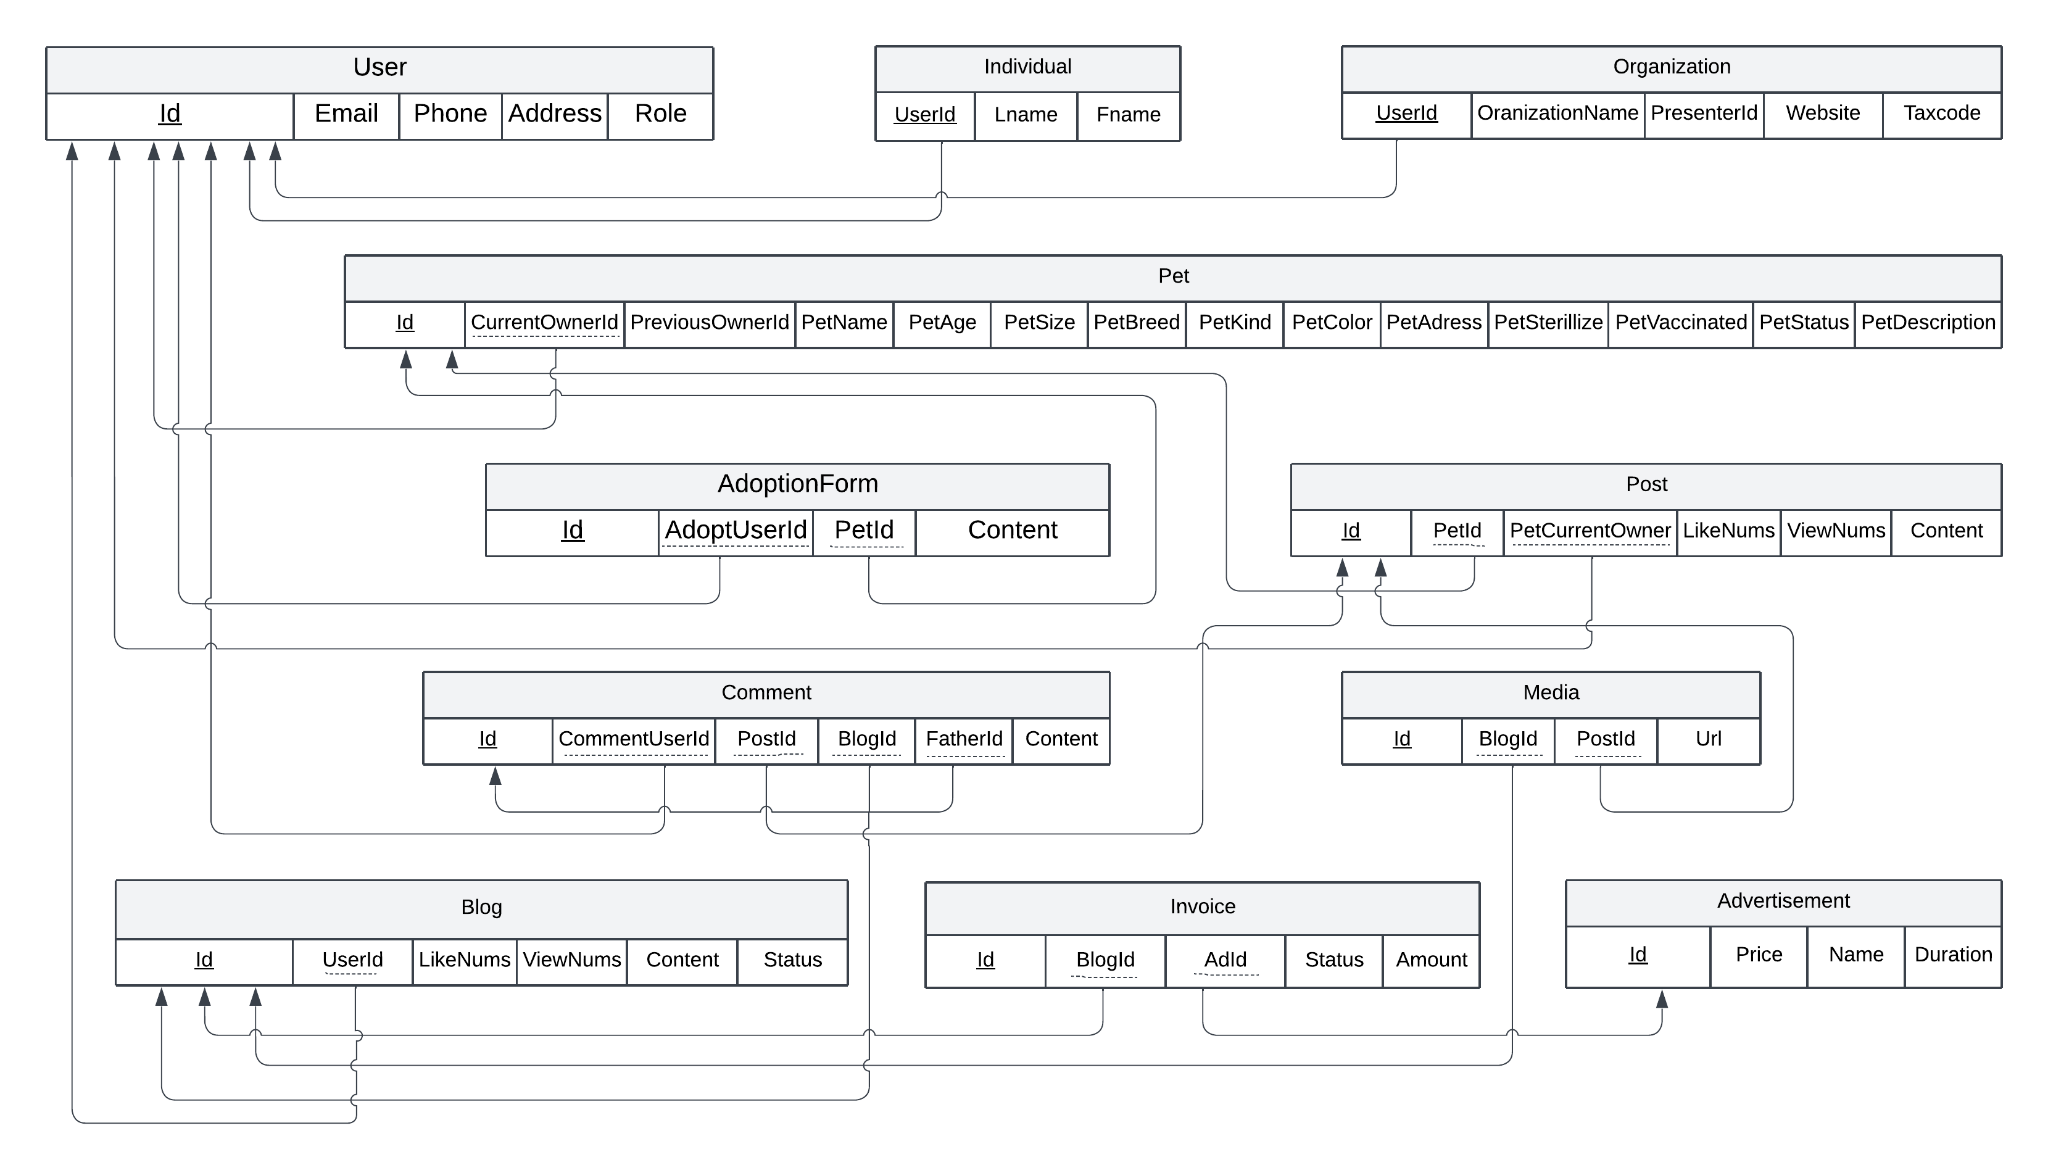
\includegraphics[width=0.8\textwidth]{Figures/relational_schema.png}
\caption{Relational schema}
\end{figure}

In \emph{Figure 55}, the excluded attributes are presented fully to
ensure the integrity of the database. In the relational mapping process,
we implement a simplified technique for the 3-way relationship where the
mandatory entity will take the primary key of the two optional entities
as its foreign key, avoiding creating another table causes the schema to
become unnecessarily complicated

\subsection{Physical Design}

In this phase, the conceptual transforms into the tangible, as we build the actual blueprint that mirrors the intricacies of the adoption process in real life. The Relational Schema serves as our guidepost, detailing the tables, attributes, and relationships that will form the foundation of the physical database. \textit{Figure 56} below translates abstract entities and relationships into concrete data types and optimizes storage structures.

\begin {figure}[H]
\centering
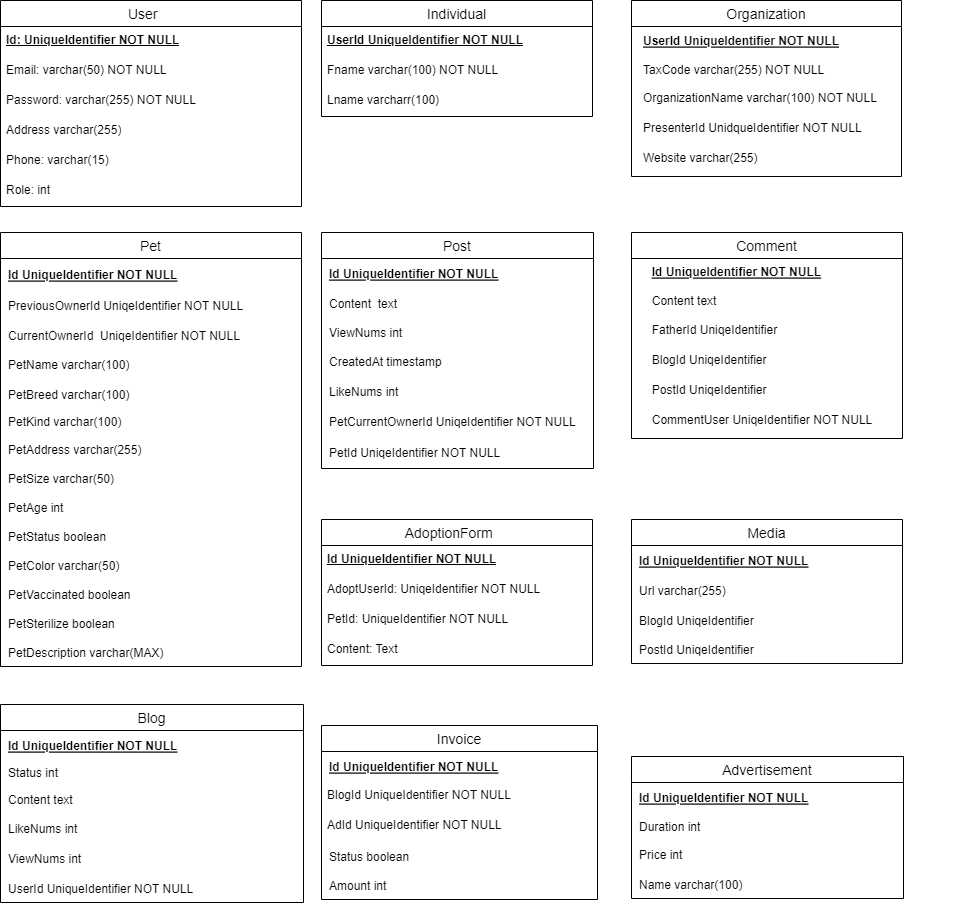
\includegraphics[width=0.8\textwidth]{Figures/physical_db.png}
\caption{Physical design}
\end{figure}




